\documentclass[11pt]{article}
\usepackage[margin=1in]{geometry}
\usepackage{amsmath,amssymb,amsthm}
\usepackage{graphicx}
\usepackage[colorlinks=true,linkcolor=blue,citecolor=blue,urlcolor=blue]{hyperref}

\newtheorem{theorem}{Theorem}[section]
\newtheorem{lemma}[theorem]{Lemma}
\newtheorem{proposition}[theorem]{Proposition}
\newtheorem{corollary}[theorem]{Corollary}
\newtheorem{definition}[theorem]{Definition}
\newtheorem{assumption}[theorem]{Assumption}
\newtheorem{conjecture}[theorem]{Conjecture}
\theoremstyle{remark}
\newtheorem{remark}[theorem]{Remark}
\newcommand{\HS}{{\rm HS}}
\newcommand{\op}{{\rm op}}
\newcommand{\Tr}{\operatorname{Tr}}

\title{Quantitative Recovery Bounds from Vacuum Clustering in Finite-Mode
Gaussian States\\
{\large (A Regularized CCR Blueprint Motivated by Split Inclusions)}\\
{\normalsize Version 2}}
\author{Lluis Eriksson\\ Independent Researcher\\ \texttt{lluiseriksson@gmail.com}}
\date{January 2026 (v1); July 2026 (v2)}

\begin{document}
\maketitle

\begin{abstract}
We prove a quantitative clustering--recovery bound for centered quasi-free
(Gaussian) states in a finite-mode bosonic CCR (Weyl) setting. Motivated by
split inclusions in algebraic quantum field theory, we work in a regularized
framework where Gaussian states are parametrized by finite covariance
matrices and a recovery map admits an explicit covariance block formula.
Using a perturbative Gaussian fidelity input and explicit coercivity bounds
for inverse covariances, we control the recovery error in terms of a vacuum
cross-correlation factor, a cross-correlation perturbation parameter, and a
recovery-error matrix norm $\|\Delta\Gamma\|_\HS$ with an explicit
quadratic+quartic structure. In a distinguished class (Family A, $X = X_0$),
this reduces to a bound in terms of the cross-block error
$\|\Delta^{(12)}\|_\HS$. We include ancillary numerical sanity checks
verifying the perturbative regime, a collar-envelope decay model, a dimension
sweep $n_1 = n_2 \in \{1,2,3\}$, and phase-diagram checks of the perturbative
domain. \emph{v2 adds:} a collar-suppressed recovery corollary making the
``clustering suppresses recovery error'' mechanism a single displayed
inequality; an upgraded discussion of the fidelity constants (the local
coefficient $1/8$ is shown numerically to be a directional benchmark, not a
uniform bound, and an empirical constant is certified on the sampled
domain); an independent verification suite in pure NumPy/SciPy implementing
the Banchi--Braunstein--Pirandola fidelity formula with closed-form anchors
(no external Gaussian-optics dependency), with all proved inequalities
tested on random draws (zero violations); positioning remarks relative
to the companion notes 2512.0060 and 2512.0101; and, aligning with
2512.0060 v2, corrected Petz-identification language (the recovery rule is
conditional reattachment, with Petz agreement only in the factorized case)
plus an explicit admissibility hypothesis for the recovered covariance.
\end{abstract}

\tableofcontents

\section{Scope, positioning, and standing regularization}

\begin{remark}[Scope note]
All results are proved in a finite-mode bosonic CCR setting (regularized
Weyl algebra on a finite-dimensional symplectic space). The Type III AQFT
setting is used only as motivation; continuum statements are formulated as
conjectural directions.
\end{remark}

\begin{remark}[Positioning]
In finite-mode continuous-variable quantum information, closed formulas for
Gaussian fidelity and many norm inequalities are standard. The contribution
of this note is an ``interface block'' that (i) packages vacuum clustering
into a cross-correlation parameter $\eta_{\rm vac}$, (ii) propagates
perturbations through a Gaussian recovery map in covariance block form, and
(iii) yields a quantitative recovery bound with explicit dependence on
coercivity and correlation parameters.
\end{remark}

\begin{remark}[Relation to the companion notes (added in v2)]
\label{rem:companions}
This note is the rigorous finite-mode core of the Gaussian
clustering--recovery program of ai.viXra:2512.0060 \cite{S0060}: there, the
reattachment/Petz reconstruction is developed for lattice vacua with
Bessel/Combes--Thomas collar suppression, and the repaired Proposition 2.14
(v2) restricts the Petz identification to a conditional reattachment with a
no-steering admissibility hypothesis. Here, by contrast, everything is finite-mode and unconditional up to one
explicit hypothesis (admissibility of the recovered covariance,
Remark~\ref{rem:adm}): the recovery rule is Definition~\ref{def:rec} taken
as an explicit covariance-level reattachment map -- \emph{not} identified
with the general Petz map (Remark~\ref{rem:petz}), in the same spirit as
0060 v2's repaired Proposition 2.14. The non-Gaussian
extension of the same bridge is conjectured via conditional mutual
information in ai.viXra:2512.0101 \cite{S0101}; Conjecture~\ref{conj:t3}
below is the Type~III counterpart. The three notes are complementary layers
of one program: lattice-Gaussian (0060), finite-mode rigorous core (this
note), non-Gaussian/CMI (0101).
\end{remark}

\begin{table}[h]
\centering
\caption{Parameter dictionary (reading aid).}
\begin{tabular}{lll}
\hline
Symbol & Meaning & Where used \\
\hline
$\epsilon$ & coercivity margin for $A$ relative to $A_0$ & Theorem~\ref{thm:main} \\
$\eta_{\rm vac}$ & reference cross-correlation factor & Definition~\ref{def:etavac} \\
$\delta$ & cross-correlation perturbation parameter & Definition~\ref{def:delta} \\
$\kappa$ & $\epsilon^{-1/2}(\eta_{\rm vac} + \delta)$ & Theorem~\ref{thm:main} \\
$\Phi$ & prefactor $(1-\kappa)^{-1}\min(\epsilon c_1, c_2)^{-1}$ & Theorem~\ref{thm:main} \\
$\Delta\Gamma$ & covariance recovery error $\Gamma - \tilde\Gamma$ & Theorem~\ref{thm:main} \\
$\Delta^{(12)}$ & cross-block error $X - \tilde X$ & Definition~\ref{def:d12} \\
\hline
\end{tabular}
\end{table}

\section{Finite-mode CCR Gaussian framework}

\subsection{Quadrature ordering and symplectic form}
\begin{remark}[Ordering convention]
Throughout, we use the standard continuous-variable ordering
$(x_1,\dots,x_N,p_1,\dots,p_N)$, so that
\[
\Omega = \begin{pmatrix} 0 & I \\ -I & 0 \end{pmatrix}.
\]
\end{remark}

\subsection{Finite symplectic space and Weyl algebra}
Let $S \simeq \mathbb{R}^{2N}$ be a real symplectic vector space with
symplectic form $\Omega$. The finite-mode Weyl algebra is generated by Weyl
operators $W(z)$, $z \in S$, satisfying
$W(z)W(z') = e^{-\frac{i}{2}\Omega(z,z')} W(z+z')$.

\subsection{Quasi-free states and covariance matrices}
\begin{definition}[Covariance and uncertainty condition]
A centered quasi-free state is specified by a real symmetric covariance
matrix $\Gamma \in \mathbb{R}^{2N\times 2N}$ satisfying
$\Gamma + \frac{i}{2}\Omega \succeq 0$.
\end{definition}

\begin{assumption}[Uniform positivity in the regularized regime]
\label{ass:pos}
All covariance blocks under consideration are strictly positive and bounded.
In particular, for the reference covariance blocks defined below, there
exist $c_1, c_2 > 0$ such that $A_0 \succeq c_1 \mathbf{1}$ and
$B_0 \succeq c_2 \mathbf{1}$.
\end{assumption}

\begin{remark}[Norm conventions]
For a real matrix $M$, $\|M\|_\HS := \sqrt{\Tr(M^T M)}$ and $\|M\|_\op$
denotes the operator norm (largest singular value).
\end{remark}

\begin{definition}[Uhlmann fidelity]
For density operators $\rho, \sigma$ on the same finite-dimensional Hilbert
space, define $F(\rho,\sigma) := \|\sqrt{\rho}\sqrt{\sigma}\|_1^2$. We write
$F(\omega_1,\omega_2)$ for the fidelity of the corresponding density
operators.
\end{definition}

\begin{remark}[Covariance convention and numerical fidelity (updated in v2)]
\label{rem:numconv}
We use the convention that physical covariances satisfy
$\Gamma + \frac{i\hbar}{2}\Omega \succeq 0$ and work with $\hbar = 1$. In v1
all numerical fidelities were evaluated with
\texttt{thewalrus.quantum.fidelity} (\texttt{hbar=1.0}). In v2 the
verification suite instead implements the closed
Banchi--Braunstein--Pirandola formula \cite{BBP} directly in NumPy/SciPy
(no external Gaussian-optics dependency) and certifies the implementation
against exact closed-form anchors: single-mode pairs via the
Marian--Marian formula \cite{Marian}, pure-state overlaps
($F(\mathrm{vac}, S(r)\mathrm{vac}) = 1/\cosh r$), the correlated two-mode
squeezed vacuum ($F(\mathrm{vac}^{\otimes 2}, \mathrm{TMSV}(r)) =
1/\cosh^2 r$), multiplicativity, and symplectic invariance; all anchors
agree to $10^{-10}$. When \texttt{thewalrus} is installed the suite runs an
optional cross-check.
\end{remark}

\subsection{Bipartition and block form}
Fix a bipartition $S = S_1 \oplus S_2$ with dimensions $2n_1$ and $2n_2$.
Write
\[
\Gamma = \begin{pmatrix} A & X \\ X^T & B \end{pmatrix},
\qquad
\Gamma_0 = \begin{pmatrix} A_0 & X_0 \\ X_0^T & B_0 \end{pmatrix}.
\]

\section{Gaussian recovery in block form}
\begin{definition}[Gaussian recovery map (covariance-level)]
\label{def:rec}
Given a centered reference covariance $\Gamma_0$ and a centered input
covariance $\Gamma$ as above, define the recovered covariance
$\tilde\Gamma$ by
\[
\tilde A = A, \qquad
\tilde X = A A_0^{-1} X_0, \qquad
\tilde B = B_0 + X_0^T A_0^{-1} (A - A_0) A_0^{-1} X_0 .
\]
\end{definition}

\begin{remark}[Relation to Petz recovery; corrected in v2]
\label{rem:petz}
Definition~\ref{def:rec} is the covariance-level \emph{conditional
reattachment} rule used in this paper. It coincides with the Petz output in
the factorized-reference case $X_0 = 0$, and may approximate the Gaussian
Petz output in strongly mixed, weak-correlation regimes, but it is \emph{not}
the Petz recovery map for general correlated Gaussian references: for
correlated references the Petz map does not preserve the input marginal, and
for a pure reference it returns the reference for every input (the failure
mode identified and repaired in 2512.0060 v2 \cite{S0060}). The main
results below use Definition~\ref{def:rec} only as an explicit
covariance-level reconstruction rule; see Appendix~A.
\end{remark}

\begin{remark}[Admissibility convention (added in v2)]
\label{rem:adm}
Throughout, Definition~\ref{def:rec} is used only on inputs for which the
recovered matrix is a valid covariance,
$\tilde\Gamma + \frac{i}{2}\Omega \succeq 0$; equivalently, the
reconstruction is a covariance-level rule on its admissible domain. This is
the finite-mode counterpart of the admissibility/no-steering hypothesis of
2512.0060 v2 \cite{S0060}. The verification suite checks this condition on
every draw (Section~\ref{sec:verif}).
\end{remark}

\section{Clustering input: vacuum cross-correlation and perturbations}
\begin{definition}[Vacuum cross-correlation factor]
\label{def:etavac}
$\eta_{\rm vac} := \| A_0^{-1/2} X_0 B_0^{-1/2} \|_\op$.
\end{definition}

\begin{definition}[Cross-correlation perturbation parameter]
\label{def:delta}
$\delta := \| A_0^{-1/2} (X - X_0) B_0^{-1/2} \|_\op$.
\end{definition}

\begin{remark}[Bessel-type collar envelope (motivational interface)]
In massive relativistic settings, equal-time correlators admit envelopes
controlled by modified Bessel functions $K_\nu(mr)$ with large-$mr$
asymptotics $K_\nu(mr) \sim \sqrt{\pi/(2mr)}\, e^{-mr}$. In our finite-mode
posture, $r$ is a collar parameter controlling the magnitude of $X_0$, and
our sanity checks use the model envelope
$\|X_0(r)\|_\op \propto (mr)^p K_\nu(mr)$.
\end{remark}

\section{Gaussian fidelity control (perturbative regime)}
\begin{lemma}[Perturbative Gaussian fidelity bound (imported, constants on a
compact set)]
\label{lem:fid}
Let $\omega_1, \omega_2$ be centered Gaussian states with covariances
$\Gamma_1 \succ 0$ and $\Gamma_2$. Define
$K := \Gamma_1^{-1/2}(\Gamma_1 - \Gamma_2)\Gamma_1^{-1/2}$. Assume
$\|K\|_\op \le \frac12$. Then there exist constants $C_2, C_4 > 0$,
depending only on the fixed finite-mode regularization (in particular on
the total mode number $N$) and on coercivity bounds of the form
$\Gamma_1 \succeq c\,\mathbf{1}$, such that
\[
1 - F(\omega_1, \omega_2) \le C_2 \|K\|_\HS^2 + C_4 \|K\|_\HS^4 .
\]
In particular, there exists $C > 0$ with the same dependence such that if
$\|K\|_\HS \le 1$ then $1 - F(\omega_1,\omega_2) \le C \|K\|_\HS^2$.
\end{lemma}

\begin{remark}[Reference and empirical constants (upgraded in v2)]
\label{rem:constants}
Closed formulas for the fidelity of Gaussian states and perturbative
expansions are standard; see \cite{BBP, Weedbrook, Serafini}.
Lemma~\ref{lem:fid} is used as a local perturbative input; we do not
optimize constants. \emph{v2 adds two quantitative facts from the
verification suite (Section~\ref{sec:verif}).} First, the local Taylor
coefficient $1/8$ suggested by expansions of the closed fidelity formula is
a \emph{directional benchmark, not a uniform bound}: across 450 random
Family-A draws ($n_1 = n_2 \in \{1,2,3\}$), the ratio
$(1-F)/\bigl(\tfrac18\|K\|_\HS^2\bigr)$ reaches $1.142$ -- and the worst
case occurs at $\|K\|_\HS \approx 2\times 10^{-3}$, i.e.\ in the local
regime, so the excess is directional rather than higher-order. Second, on
the sampled compact domain the suite certifies the empirical constant
$C_2^{\rm emp} \approx 0.143$, i.e.
$1 - F \le C_2^{\rm emp}\, \|K\|_\HS^2$ across all draws, consistent with
(and instantiating) the existence claim of Lemma~\ref{lem:fid}.
\end{remark}

\section{Main theorem: clustering--recovery bridge (Route 1)}
\begin{definition}[Partial local excitation]
\label{def:ple}
We say $\omega$ is a partial local excitation (relative to the bipartition)
if $B = B_0$.
\end{definition}

\begin{definition}[Recovery cross-block error]
\label{def:d12}
With $\tilde X$ as in Definition~\ref{def:rec}, define
$\Delta^{(12)} := X - \tilde X = X - A A_0^{-1} X_0$.
\end{definition}

\begin{lemma}[From relative perturbation to a uniform lower bound]
\label{lem:eps}
If $\|A_0^{-1/2}(A - A_0)A_0^{-1/2}\|_\op \le 1 - \epsilon$ with
$\epsilon \in (0,1)$, then $A \succeq \epsilon A_0$.
\end{lemma}
\begin{proof}
Let $E := A_0^{-1/2}(A - A_0)A_0^{-1/2}$. The hypothesis implies
$E \succeq -(1-\epsilon)\mathbf{1}$, hence
$A = A_0^{1/2}(\mathbf{1} + E)A_0^{1/2} \succeq \epsilon A_0$.
\end{proof}

\begin{lemma}[Block structure of the recovery covariance error]
\label{lem:block}
Assume $B = B_0$ and $\tilde\Gamma$ is given by Definition~\ref{def:rec}.
Then $\Delta\Gamma := \Gamma - \tilde\Gamma$ has block form
\[
\Delta\Gamma = \begin{pmatrix} 0 & \Delta^{(12)} \\
(\Delta^{(12)})^T & \Delta^{(22)} \end{pmatrix},
\qquad
\Delta^{(22)} = B_0 - \tilde B = -X_0^T A_0^{-1}(A - A_0)A_0^{-1} X_0 .
\]
In particular,
$\|\Delta\Gamma\|_\HS^2 = 2\|\Delta^{(12)}\|_\HS^2 + \|\Delta^{(22)}\|_\HS^2$,
and
$\|\Delta^{(22)}\|_\HS \le \|A - A_0\|_\HS \|A_0^{-1}X_0\|_\op^2$.
\end{lemma}
\begin{proof}
The block form is immediate from $\tilde A = A$ and $B = B_0$. For the
estimate, use $\|UVW\|_\HS \le \|U\|_\op \|V\|_\HS \|W\|_\op$ with
$U = X_0^T A_0^{-1}$, $V = A - A_0$, $W = A_0^{-1}X_0$.
\end{proof}

\begin{proposition}[Coercivity bound for $\|\Gamma^{-1}\|_\op$ with no hidden
constants]
\label{prop:coerc}
Let $B_0 \succ 0$ and $\Gamma = \begin{pmatrix} A & X \\ X^T & B_0
\end{pmatrix}$ with $A \succ 0$. Define
$\eta_\omega := \|A^{-1/2} X B_0^{-1/2}\|_\op$. If $\eta_\omega < 1$, then
\[
\Gamma \succeq (1 - \eta_\omega)
\begin{pmatrix} A & 0 \\ 0 & B_0 \end{pmatrix},
\qquad\text{hence}\qquad
\|\Gamma^{-1}\|_\op \le
\frac{1}{(1-\eta_\omega)\min(\lambda_{\min}(A), \lambda_{\min}(B_0))}.
\]
In particular, if $A \succeq \epsilon A_0$, $A_0 \succeq c_1\mathbf{1}$ and
$B_0 \succeq c_2\mathbf{1}$, then
$\|\Gamma^{-1}\|_\op \le \bigl[(1-\eta_\omega)\min(\epsilon c_1, c_2)\bigr]^{-1}$.
\end{proposition}
\begin{proof}
Let $u \in \mathbb{R}^{2n_1}$, $v \in \mathbb{R}^{2n_2}$ and set
$a := A^{1/2}u$, $b := B_0^{1/2}v$. Then
\[
\begin{pmatrix} u \\ v \end{pmatrix}^{\!T}
\Gamma
\begin{pmatrix} u \\ v \end{pmatrix}
= \|a\|_2^2 + 2\, a^T \bigl(A^{-1/2} X B_0^{-1/2}\bigr) b + \|b\|_2^2 .
\]
By Cauchy--Schwarz,
$2\, a^T (A^{-1/2}XB_0^{-1/2}) b \ge -2\eta_\omega \|a\|_2 \|b\|_2 \ge
-\eta_\omega(\|a\|_2^2 + \|b\|_2^2)$, which proves the Loewner bound; taking
minimal eigenvalues yields the inverse-norm bound.
\end{proof}

\begin{proposition}[Bounding $\eta_\omega$ by $\eta_{\rm vac} + \delta$]
\label{prop:eta}
Assume $A \succeq \epsilon A_0$ with $\epsilon \in (0,1)$. Then
$\eta_\omega \le \epsilon^{-1/2}\|A_0^{-1/2}XB_0^{-1/2}\|_\op
\le \epsilon^{-1/2}(\eta_{\rm vac} + \delta)$.
\end{proposition}
\begin{proof}
Since $A \succeq \epsilon A_0$, $\|A^{-1/2}A_0^{1/2}\|_\op \le
\epsilon^{-1/2}$; submultiplicativity and the triangle inequality for
$X = X_0 + (X - X_0)$ finish the proof.
\end{proof}

\begin{proposition}[A simple sufficient condition for the perturbative regime]
\label{prop:suff}
If $\|\Gamma^{-1}\|_\op \|\Delta\Gamma\|_\HS \le \frac12$, then
$\|K\|_\op \le \frac12$ and Lemma~\ref{lem:fid} applies.
\end{proposition}
\begin{proof}
$\|K\|_\op = \|\Gamma^{-1/2}\Delta\Gamma\,\Gamma^{-1/2}\|_\op \le
\|\Gamma^{-1}\|_\op\|\Delta\Gamma\|_\op \le
\|\Gamma^{-1}\|_\op\|\Delta\Gamma\|_\HS$.
\end{proof}

\begin{theorem}[Clustering--recovery bridge (finite-mode Gaussian; Route 1,
quadratic+quartic)]
\label{thm:main}
Let $\omega_0$ be a centered reference Gaussian state with covariance
$\Gamma_0$ and blocks $(A_0, X_0, B_0)$ satisfying
Assumption~\ref{ass:pos}. Let $\omega$ be a centered Gaussian state with
covariance $\Gamma$ and blocks $(A, X, B)$ such that $\omega$ is a partial
local excitation (Definition~\ref{def:ple}), i.e.\ $B = B_0$. Assume there
exists $\epsilon \in (0,1)$ such that
$\|A_0^{-1/2}(A - A_0)A_0^{-1/2}\|_\op \le 1 - \epsilon$, and define
$\kappa := \epsilon^{-1/2}(\eta_{\rm vac} + \delta)$. Assume $\kappa < 1$.
Let $\tilde\omega$ be the recovered centered Gaussian state with covariance
$\tilde\Gamma$ given by Definition~\ref{def:rec}. Assume in addition that the recovered covariance $\tilde\Gamma$ is
physical, $\tilde\Gamma + \frac{i}{2}\Omega \succeq 0$
(Remark~\ref{rem:adm}), and that
$\|K\|_\op \le \frac12$, where
$K := \Gamma^{-1/2}(\Gamma - \tilde\Gamma)\Gamma^{-1/2}$ (for instance, it
suffices that Proposition~\ref{prop:suff} holds). Then, with
$\Delta\Gamma := \Gamma - \tilde\Gamma$,
\[
1 - F(\omega, \tilde\omega) \le
C_2\, \Phi^2 \|\Delta\Gamma\|_\HS^2 + C_4\, \Phi^4 \|\Delta\Gamma\|_\HS^4,
\qquad
\Phi := \frac{1}{(1-\kappa)\min(\epsilon c_1, c_2)},
\]
where $C_2, C_4 > 0$ are the constants from Lemma~\ref{lem:fid}.
\end{theorem}
\begin{proof}
By submultiplicativity and $\|M\|_\op \le \|M\|_\HS$,
$\|K\|_\HS \le \|\Gamma^{-1}\|_\op \|\Delta\Gamma\|_\HS$. By
Lemma~\ref{lem:eps}, $A \succeq \epsilon A_0$, and
Proposition~\ref{prop:eta} yields $\eta_\omega \le \kappa < 1$. Therefore
Proposition~\ref{prop:coerc} gives $\|\Gamma^{-1}\|_\op \le \Phi$. Insert
into Lemma~\ref{lem:fid}.
\end{proof}

\begin{remark}[Coarsenings of the correlation denominator]
For $\kappa \in [0,1)$, $1 - \kappa^2 = (1-\kappa)(1+\kappa) \le
2(1-\kappa)$, hence $(1-\kappa)^{-m} \le 2^m (1-\kappa^2)^{-m}$ for
$m = 1, 2, 4$; prefactors may equivalently be rewritten in terms of
$(1-\kappa^2)$ at the cost of numerical constants. We keep the explicit
$(1-\kappa)$ form matching Proposition~\ref{prop:coerc}.
\end{remark}

\begin{corollary}[Purely quadratic regime]
\label{cor:quad}
Under the hypotheses of Theorem~\ref{thm:main}, if additionally
$\|K\|_\HS \le 1$, then
$1 - F(\omega,\tilde\omega) \le C\, \Phi^2 \|\Delta\Gamma\|_\HS^2$, with
$C$ from Lemma~\ref{lem:fid} and $\Phi$ as in Theorem~\ref{thm:main}.
\end{corollary}

\begin{corollary}[Reduction to $\|\Delta^{(12)}\|_\HS$ in the Family A case]
\label{cor:famA}
Assume the hypotheses of Theorem~\ref{thm:main} and, in addition,
$X = X_0$. Then one may take
$C_\Delta := \sqrt{2 + \|X_0^T A_0^{-1}\|_\op^2}$ so that
$\|\Delta\Gamma\|_\HS \le C_\Delta \|\Delta^{(12)}\|_\HS$.
\end{corollary}
\begin{proof}
If $X = X_0$, then $\Delta^{(12)} = X_0 - AA_0^{-1}X_0 =
-(A - A_0)A_0^{-1}X_0$. Lemma~\ref{lem:block} gives
$\Delta^{(22)} = X_0^T A_0^{-1}\Delta^{(12)}$, hence
$\|\Delta^{(22)}\|_\HS \le \|X_0^T A_0^{-1}\|_\op \|\Delta^{(12)}\|_\HS$;
substitute into
$\|\Delta\Gamma\|_\HS^2 = 2\|\Delta^{(12)}\|_\HS^2 + \|\Delta^{(22)}\|_\HS^2$.
\end{proof}

\begin{corollary}[Collar-suppressed recovery (added in v2)]
\label{cor:collar}
Assume the hypotheses of Theorem~\ref{thm:main} with $X = X_0$ (Family A,
so $\delta = 0$) and $\|K\|_\HS \le 1$. Then
\[
\boxed{\;
1 - F(\omega, \tilde\omega) \;\le\;
C\, \Phi^2\, C_\Delta^2\;
\|A - A_0\|_\HS^2\; \bigl\|A_0^{-1} X_0\bigr\|_\op^2
\;}
\]
with $C$ from Lemma~\ref{lem:fid}, $\Phi$ from Theorem~\ref{thm:main} and
$C_\Delta$ from Corollary~\ref{cor:famA}. In particular, under a collar
envelope $\|X_0(r)\|_\op \propto (mr)^p K_\nu(mr)$, the right-hand side
inherits the squared envelope $e^{-2mr}$ (up to the polynomial factor) at
fixed perturbation strength $\|A - A_0\|_\HS$: vacuum clustering suppresses
the recovery error quadratically in the correlator envelope.
\end{corollary}
\begin{proof}
$\Delta^{(12)} = -(A - A_0)A_0^{-1}X_0$ gives
$\|\Delta^{(12)}\|_\HS \le \|A - A_0\|_\HS \|A_0^{-1}X_0\|_\op$; combine
with Corollaries~\ref{cor:quad} and \ref{cor:famA}. For the envelope
statement, $\|A_0^{-1}X_0\|_\op \le \|A_0^{-1}\|_\op \|X_0\|_\op \le
c_1^{-1}\|X_0(r)\|_\op$.
\end{proof}

\section{Ancillary numerical sanity-checks}
\begin{remark}[Reproducibility and physicality checks]
The numerical experiments check physicality of both $\Gamma$ and
$\tilde\Gamma$ by verifying
$\lambda_{\min}(\Gamma + \frac{i}{2}\Omega) \ge -\tau$ and
$\lambda_{\min}(\tilde\Gamma + \frac{i}{2}\Omega) \ge -\tau$ for a fixed
tolerance $\tau > 0$.
\end{remark}

\begin{remark}[Numerical constants versus theoretical constants (updated in v2)]
Lemma~\ref{lem:fid} is stated with constants on a compact set. In the
numerical plots we additionally compare against sharper coefficients such
as $\frac18$ and $\frac{1}{48}$ suggested by local Taylor expansions of
closed Gaussian fidelity formulas; per Remark~\ref{rem:constants}, v2
quantifies their status: $\frac18$ is a directional benchmark exceeded by
up to $14\%$ in worst-case directions, and the certified empirical constant
on the sampled domain is $C_2^{\rm emp} \approx 0.143$.
\end{remark}

\subsection{Representative figures}
For readability, we keep the base sanity check figures in the main text and
move extended sweeps to Appendix~B.

\begin{figure}[h]
\centering
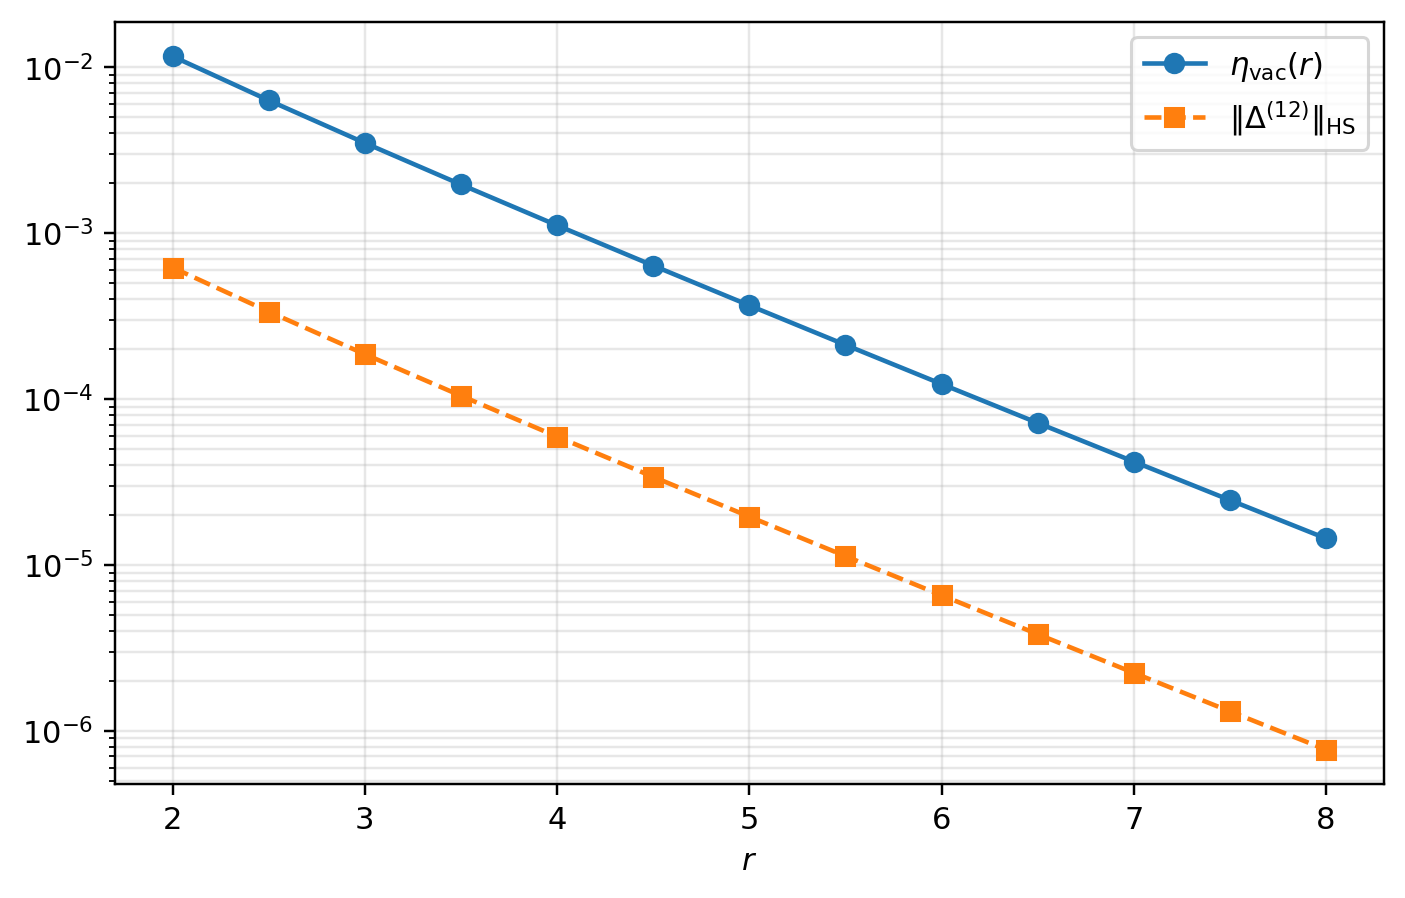
\includegraphics[width=0.72\textwidth]{fig01_base_eta_delta.png}
\caption{Base sanity check ($n_1 = n_2 = 2$): $\eta_{\rm vac}(r)$ and
$\|\Delta^{(12)}\|_\HS$ versus $r$ under a Bessel-type envelope.}
\end{figure}

\begin{figure}[h]
\centering
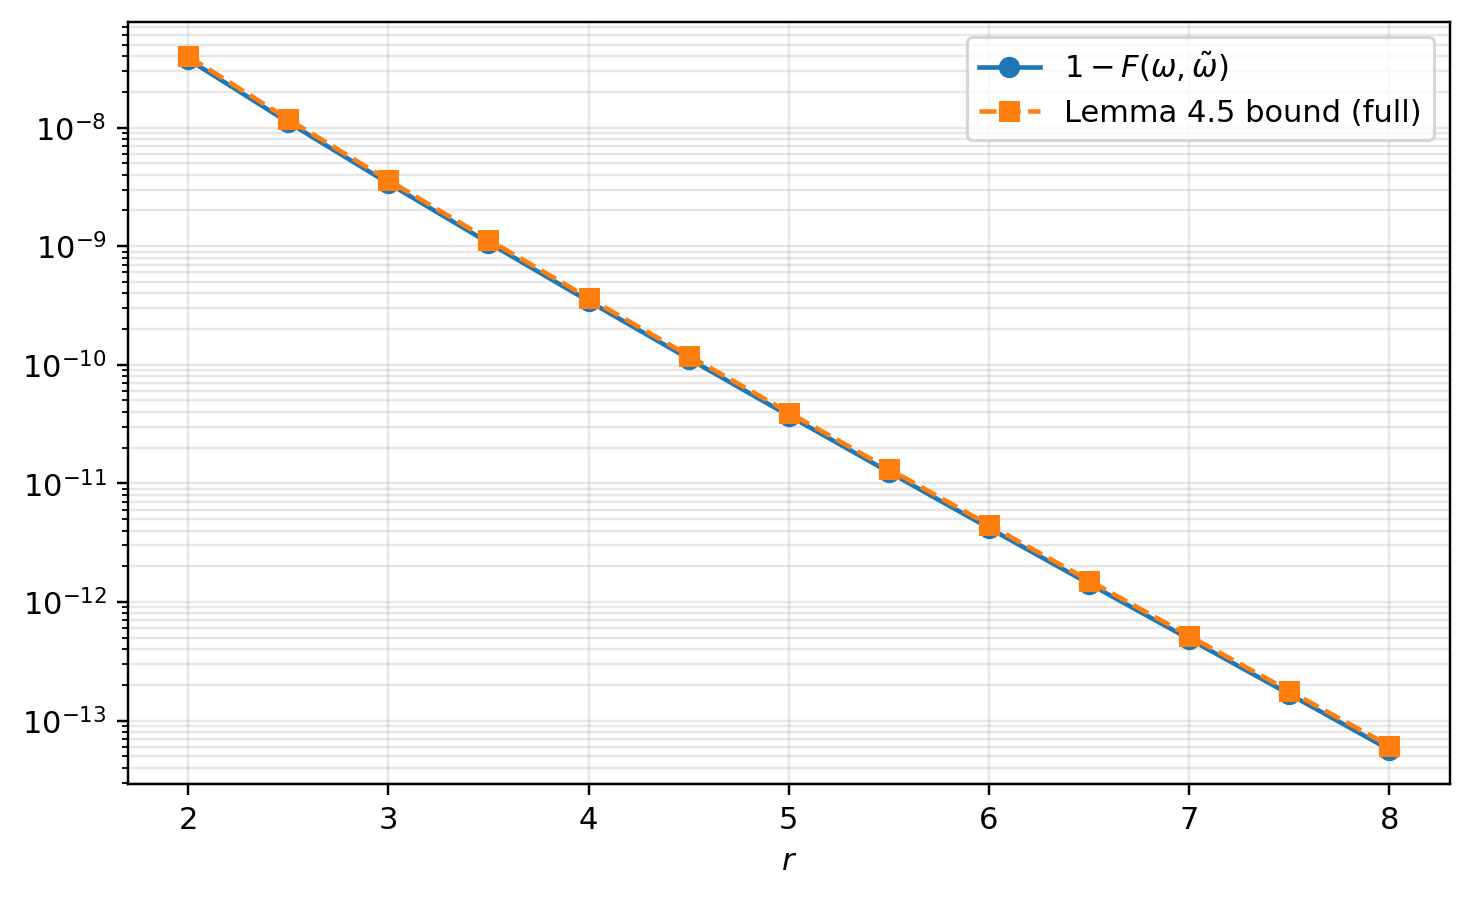
\includegraphics[width=0.72\textwidth]{fig02_base_fidelity.png}
\caption{Base sanity check ($n_1 = n_2 = 2$): $1 - F(\omega,\tilde\omega)$
versus a perturbative Gaussian fidelity benchmark.}
\end{figure}

\section{Independent verification suite (added in v2)}
\label{sec:verif}
The repository ships \texttt{verification/2601-0007/verify\_2601\_0007.py},
a pure NumPy/SciPy suite with no Gaussian-optics dependency:

\emph{(i) Certified fidelity kernel.} The Banchi--Braunstein--Pirandola
closed formula \cite{BBP} is implemented directly ($\hbar = 1$ convention
of Remark~\ref{rem:numconv}) and certified against exact anchors -- the
single-mode Marian--Marian formula \cite{Marian}, pure-state overlaps
$1/\cosh r$, the two-mode squeezed vacuum $1/\cosh^2 r$ (a correlated
multimode case), multiplicativity on products, and symplectic invariance --
all to $10^{-10}$.

\emph{(ii) Inequality suite.} On 450 random Family-A draws
($n_1 = n_2 \in \{1,2,3\}$, 150 each, physicality enforced), the suite
verifies with \emph{zero violations}: physicality of the recovered covariance
$\tilde\Gamma + \frac{i}{2}\Omega \succeq 0$ on every draw
(Remark~\ref{rem:adm}); the exact block identity and HS
decomposition of Lemma~\ref{lem:block} (machine precision); the coercivity
inequality of Proposition~\ref{prop:coerc}; the bound of
Proposition~\ref{prop:eta}; Corollary~\ref{cor:famA} with its explicit
$C_\Delta$; the norm chain
$\|K\|_\HS \le \|\Gamma^{-1}\|_\op\|\Delta\Gamma\|_\HS \le
\Phi\|\Delta\Gamma\|_\HS$; and the collar-suppressed bound of
Corollary~\ref{cor:collar}.

\emph{(iii) Constants.} The suite certifies
$C_2^{\rm emp} \approx 0.143$ on the sampled domain and locates the
worst-case direction (ratio $1.142$ against the $\frac18$ benchmark at
$\|K\|_\HS \approx 2\times 10^{-3}$; see Remark~\ref{rem:constants}).

\emph{(iv) Collar sweep.} Under the Bessel envelope of
Remark~4.1
with $r \in [2, 8]$, both $1 - F$ (from $3.9\times 10^{-6}$ to
$5.9\times 10^{-12}$) and the Corollary~\ref{cor:collar} bound (from
$1.4\times 10^{-5}$ to $1.9\times 10^{-11}$) decay monotonically, with the
bound dominating pointwise.

\section{Conjectural outlook (Type III / non-Gaussian)}
\begin{conjecture}[Type III clustering--recovery blueprint]
\label{conj:t3}
Let $\omega_0$ be the vacuum state of a massive AQFT satisfying a split
inclusion for $\mathcal{O}_1 \Subset \mathcal{O}_2$. For suitable classes
of states $\omega$ that are vacuum-like outside $\mathcal{O}_2$ and have
finite Araki relative entropy, the Petz recovery associated with the
$\omega_0$-preserving conditional expectation onto a canonical split factor
yields an estimate of the form
$1 - F(\omega, \tilde\omega) \le C\, \mathcal{C}(\mathcal{O}_1,
\mathcal{O}_2)^\gamma$, where $\mathcal{C}(\mathcal{O}_1,\mathcal{O}_2)$ is
a clustering coefficient controlled by collar width and the mass gap.
\end{conjecture}

\begin{remark}[Type III roadmap]
The transition to the Type III setting likely requires noncommutative
$L^p$ methods (e.g.\ Haagerup spaces) to express quantitative analogues of
density operators and fidelity-type functionals. In this picture,
covariance-block control in the finite-mode Gaussian setting is expected to
be replaced by bounds on relative modular operators associated with the
split factor and the $\omega_0$-preserving conditional expectation. The
CMI-based route to the same bridge is developed in \cite{S0101}.
\end{remark}

\section*{Note added in v2}
No theorem of v1 required correction: all v1 bounds, proofs and figures are
unchanged. v2 does correct the non-load-bearing \emph{Petz identification}
language of v1 (Remark~\ref{rem:petz}, Appendix~A): the covariance rule of
Definition~\ref{def:rec} is conditional reattachment, not the general Petz
map for correlated references -- aligning this note with the repaired
Proposition 2.14 of 2512.0060 v2. The theorem now also states explicitly
the admissibility hypothesis $\tilde\Gamma + \frac{i}{2}\Omega \succeq 0$
(Remark~\ref{rem:adm}), previously only enforced in the numerics. v2
further adds:
(1) Corollary~\ref{cor:collar} (collar-suppressed recovery), packaging the
main mechanism into one displayed inequality with squared-envelope decay;
(2) Remark~\ref{rem:constants}: the $\tfrac18$ Taylor coefficient is a
directional benchmark exceeded by up to $14\%$ in worst-case directions
even as $\|K\| \to 0$; an empirical constant $C_2^{\rm emp} \approx 0.143$
is certified on the sampled domain, instantiating Lemma~\ref{lem:fid};
(3) Section~\ref{sec:verif}: an independent pure-NumPy verification suite
(BBP fidelity kernel certified to $10^{-10}$ against closed-form anchors,
including a correlated two-mode case; 450 draws, zero violations of any
proved inequality; collar sweep), removing the \texttt{thewalrus}
dependency of the v1 appendix script (kept as optional cross-check);
(4) Remark~\ref{rem:companions}: positioning relative to 2512.0060 and
2512.0101 (lattice-Gaussian / finite-mode core / non-Gaussian CMI);
(5) references added: \cite{Marian}, series companions.

\appendix

\section{Appendix: conditional reattachment covariance rule (rewritten in v2)}
The v1 version of this appendix presented a ``Petz identification sketch''
arguing that Definition~\ref{def:rec} matches the Petz map by requiring
that the map (i) fixes the subsystem-1 marginal and (ii) recovers the
reference exactly. That heuristic is false in general: conditions (i)--(ii)
characterize the \emph{conditional reattachment} rule, not the Petz map,
which for correlated references does not satisfy (i), and for pure
references collapses to the reference on all inputs (2512.0060 v2
\cite{S0060}). What survives is the following: Definition~\ref{def:rec} is
the unique covariance-level map that is affine in $A$, fixes the
subsystem-1 marginal ($\tilde A = A$), and is exact on the reference
($\Gamma = \Gamma_0 \Rightarrow \tilde\Gamma = \Gamma_0$); it agrees
with the Petz output when $X_0 = 0$ (factorized reference), and its
relation to the Gaussian Petz map beyond that case is an approximation
question in strongly mixed regimes (route: Lami--Das--Wilde), not an
identity. All results of this paper use only the reattachment rule on its
admissible domain (Remark~\ref{rem:adm}).

\section{Appendix: extended figures}
\begin{figure}[h]
\centering
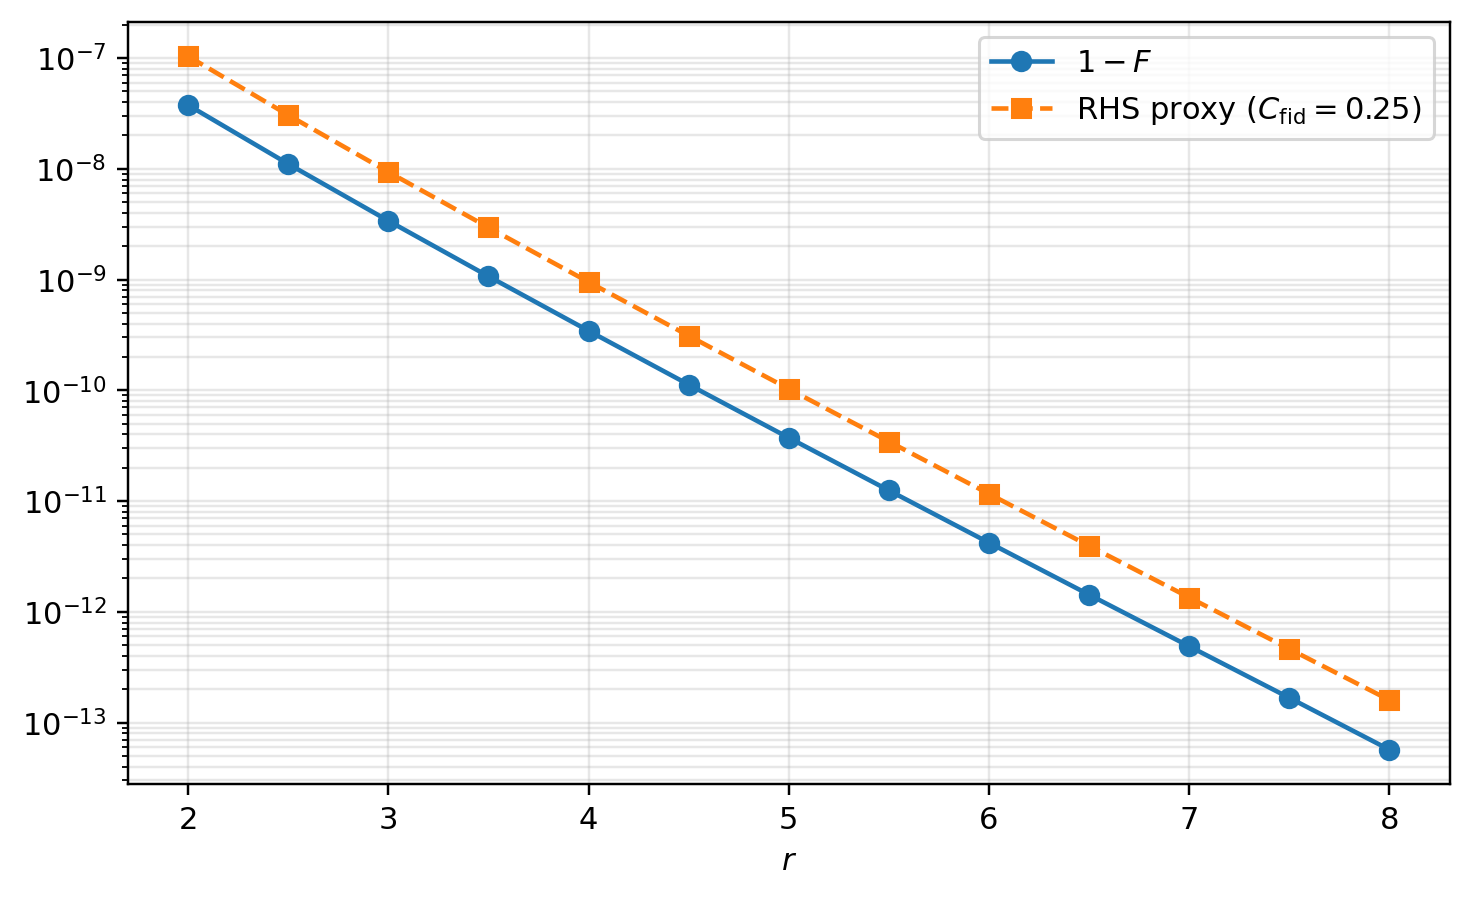
\includegraphics[width=0.7\textwidth]{fig03_rhs_proxy.png}
\caption{Base sanity check ($n_1=n_2=2$): $1-F$ versus a proxy of the RHS
scaling in Theorem~\ref{thm:main}.}
\end{figure}
\begin{figure}[h]
\centering
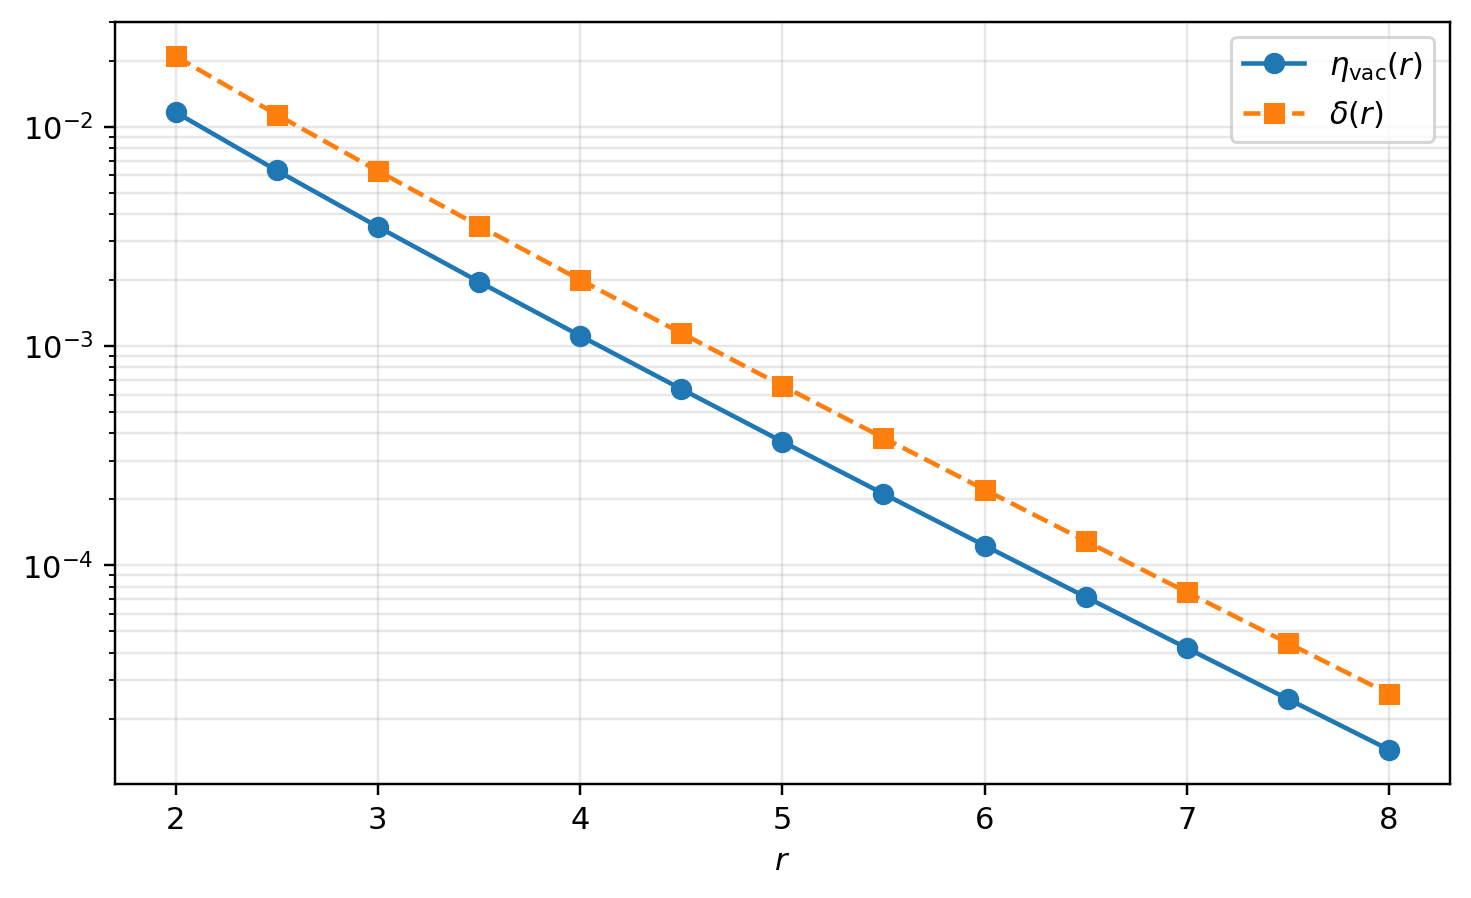
\includegraphics[width=0.7\textwidth]{fig04_familyB_delta.png}
\caption{N1 (Family B): engineered perturbation $\delta(r)$ inherits the
collar envelope and decays with $r$, alongside $\eta_{\rm vac}(r)$.}
\end{figure}
\begin{figure}[h]
\centering
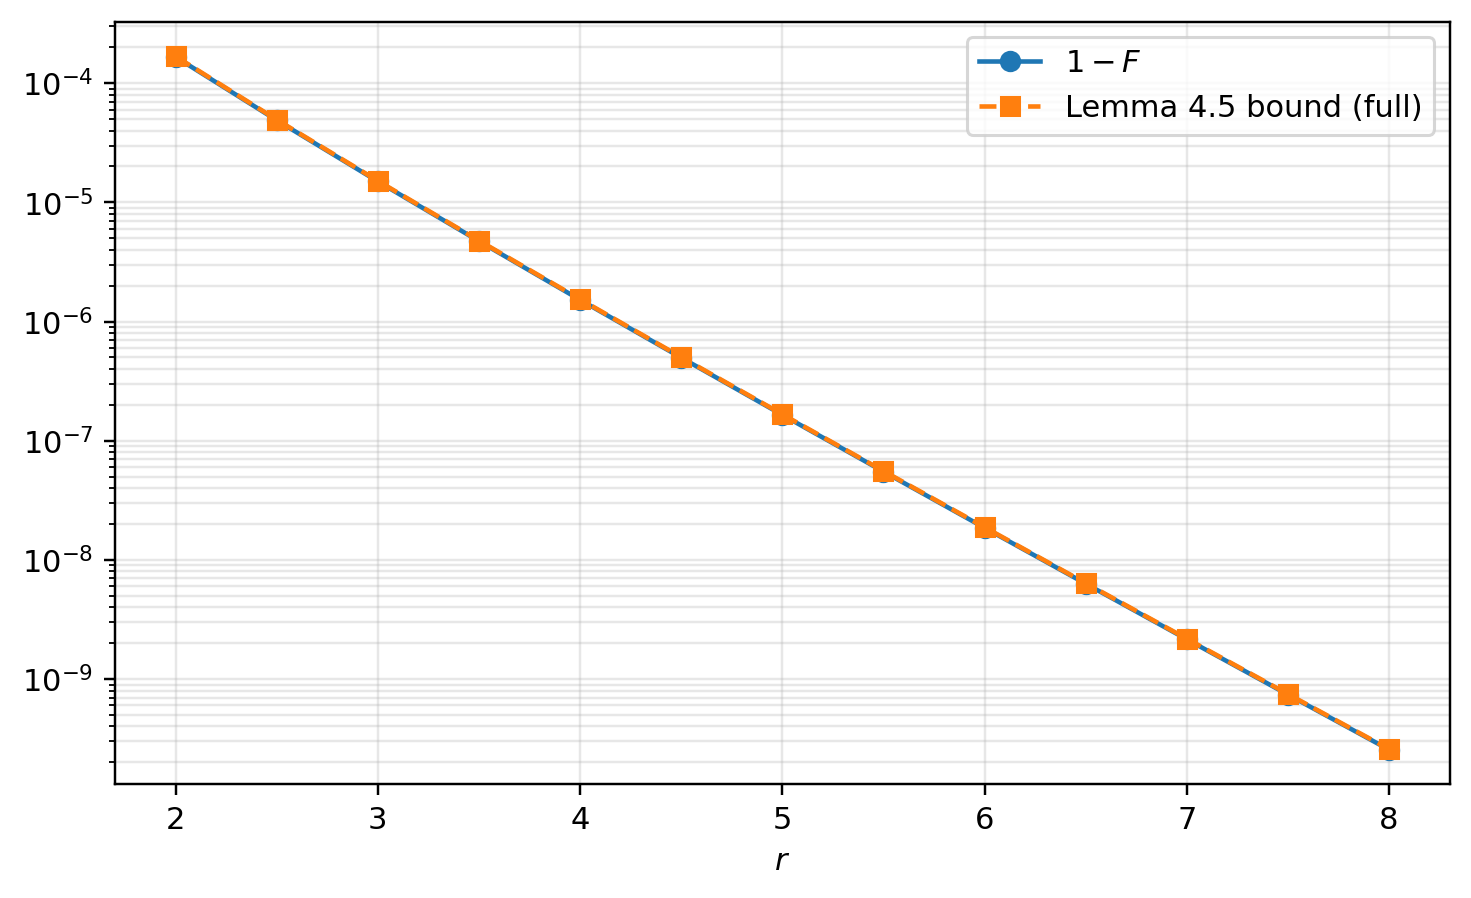
\includegraphics[width=0.7\textwidth]{fig05_familyB_fid.png}
\caption{N1: fidelity-benchmark comparison for the Family B construction.}
\end{figure}
\begin{figure}[h]
\centering
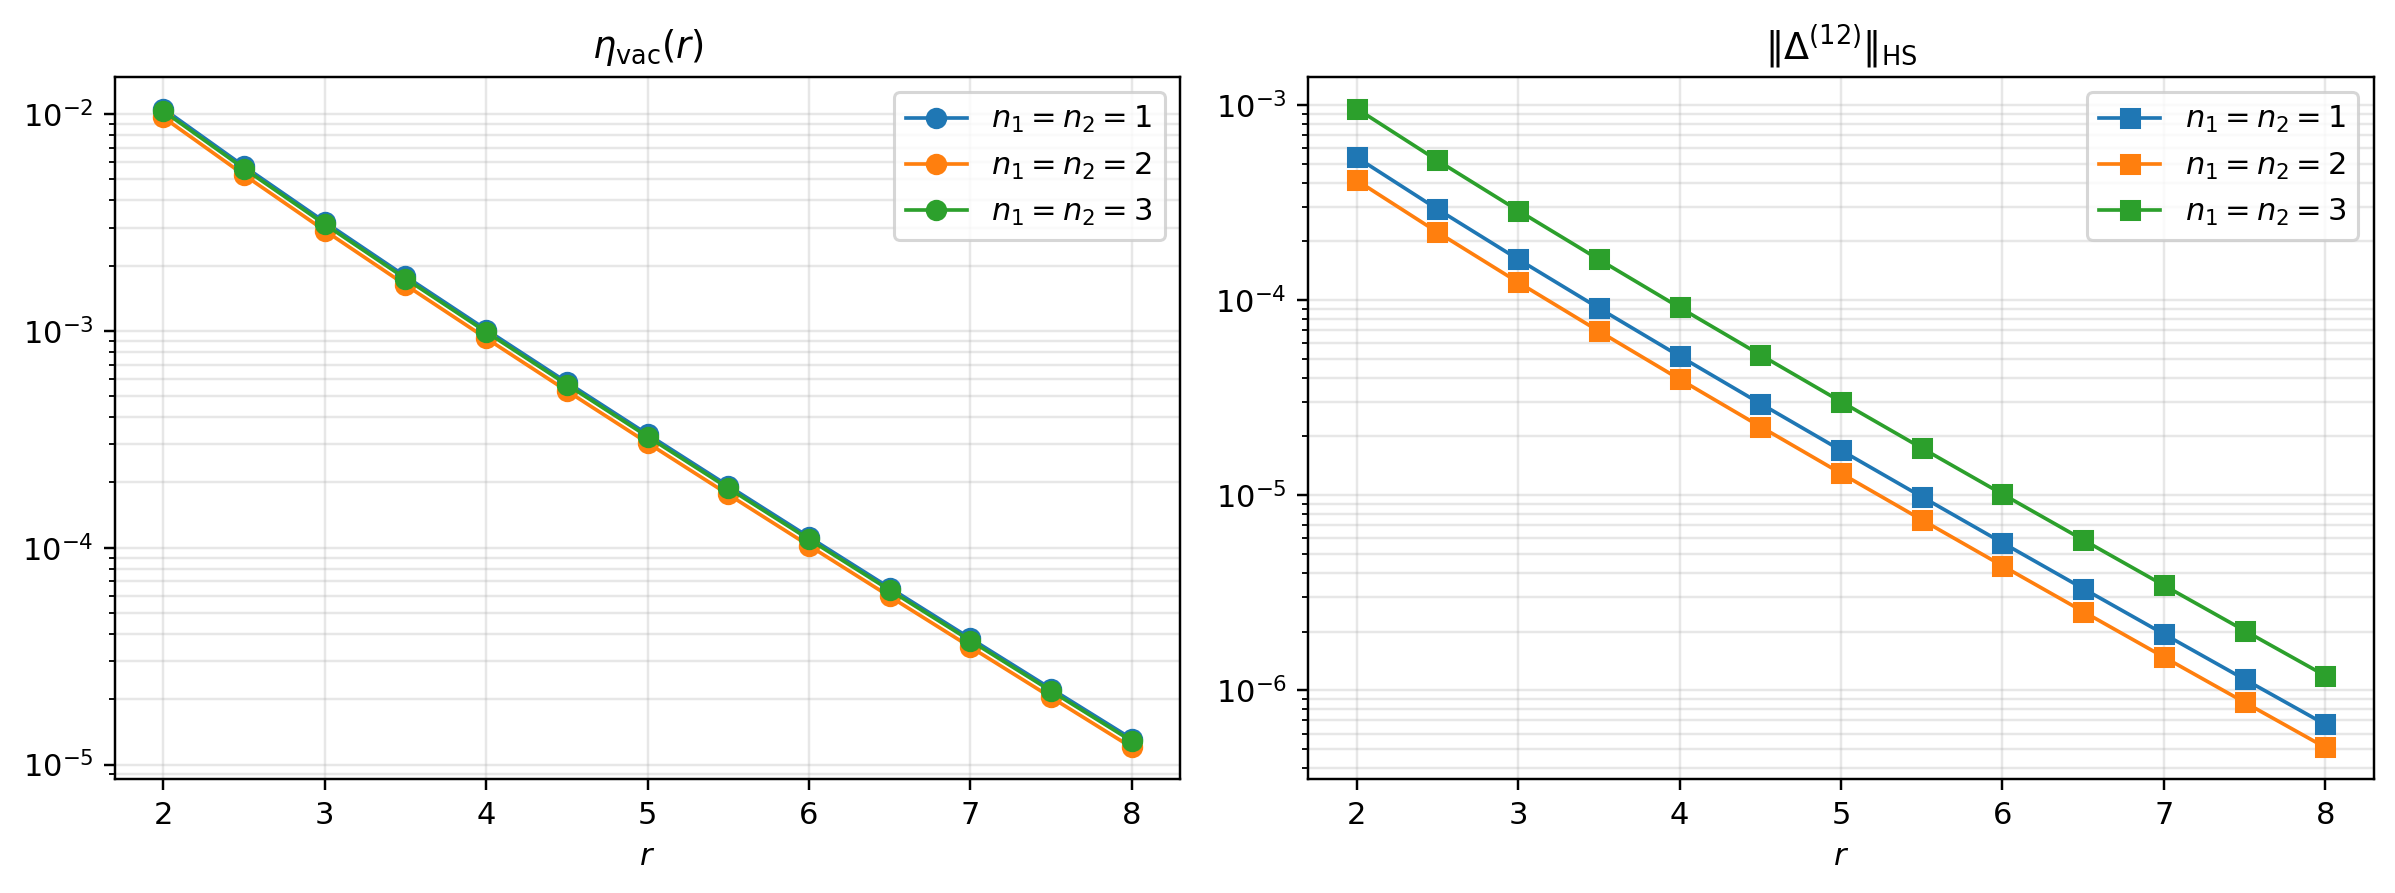
\includegraphics[width=0.75\textwidth]{fig06_dimsweep_eta.png}
\caption{N2: $\eta_{\rm vac}(r)$ and $\|\Delta^{(12)}\|_\HS$ for
$n_1 = n_2 \in \{1,2,3\}$.}
\end{figure}
\begin{figure}[h]
\centering
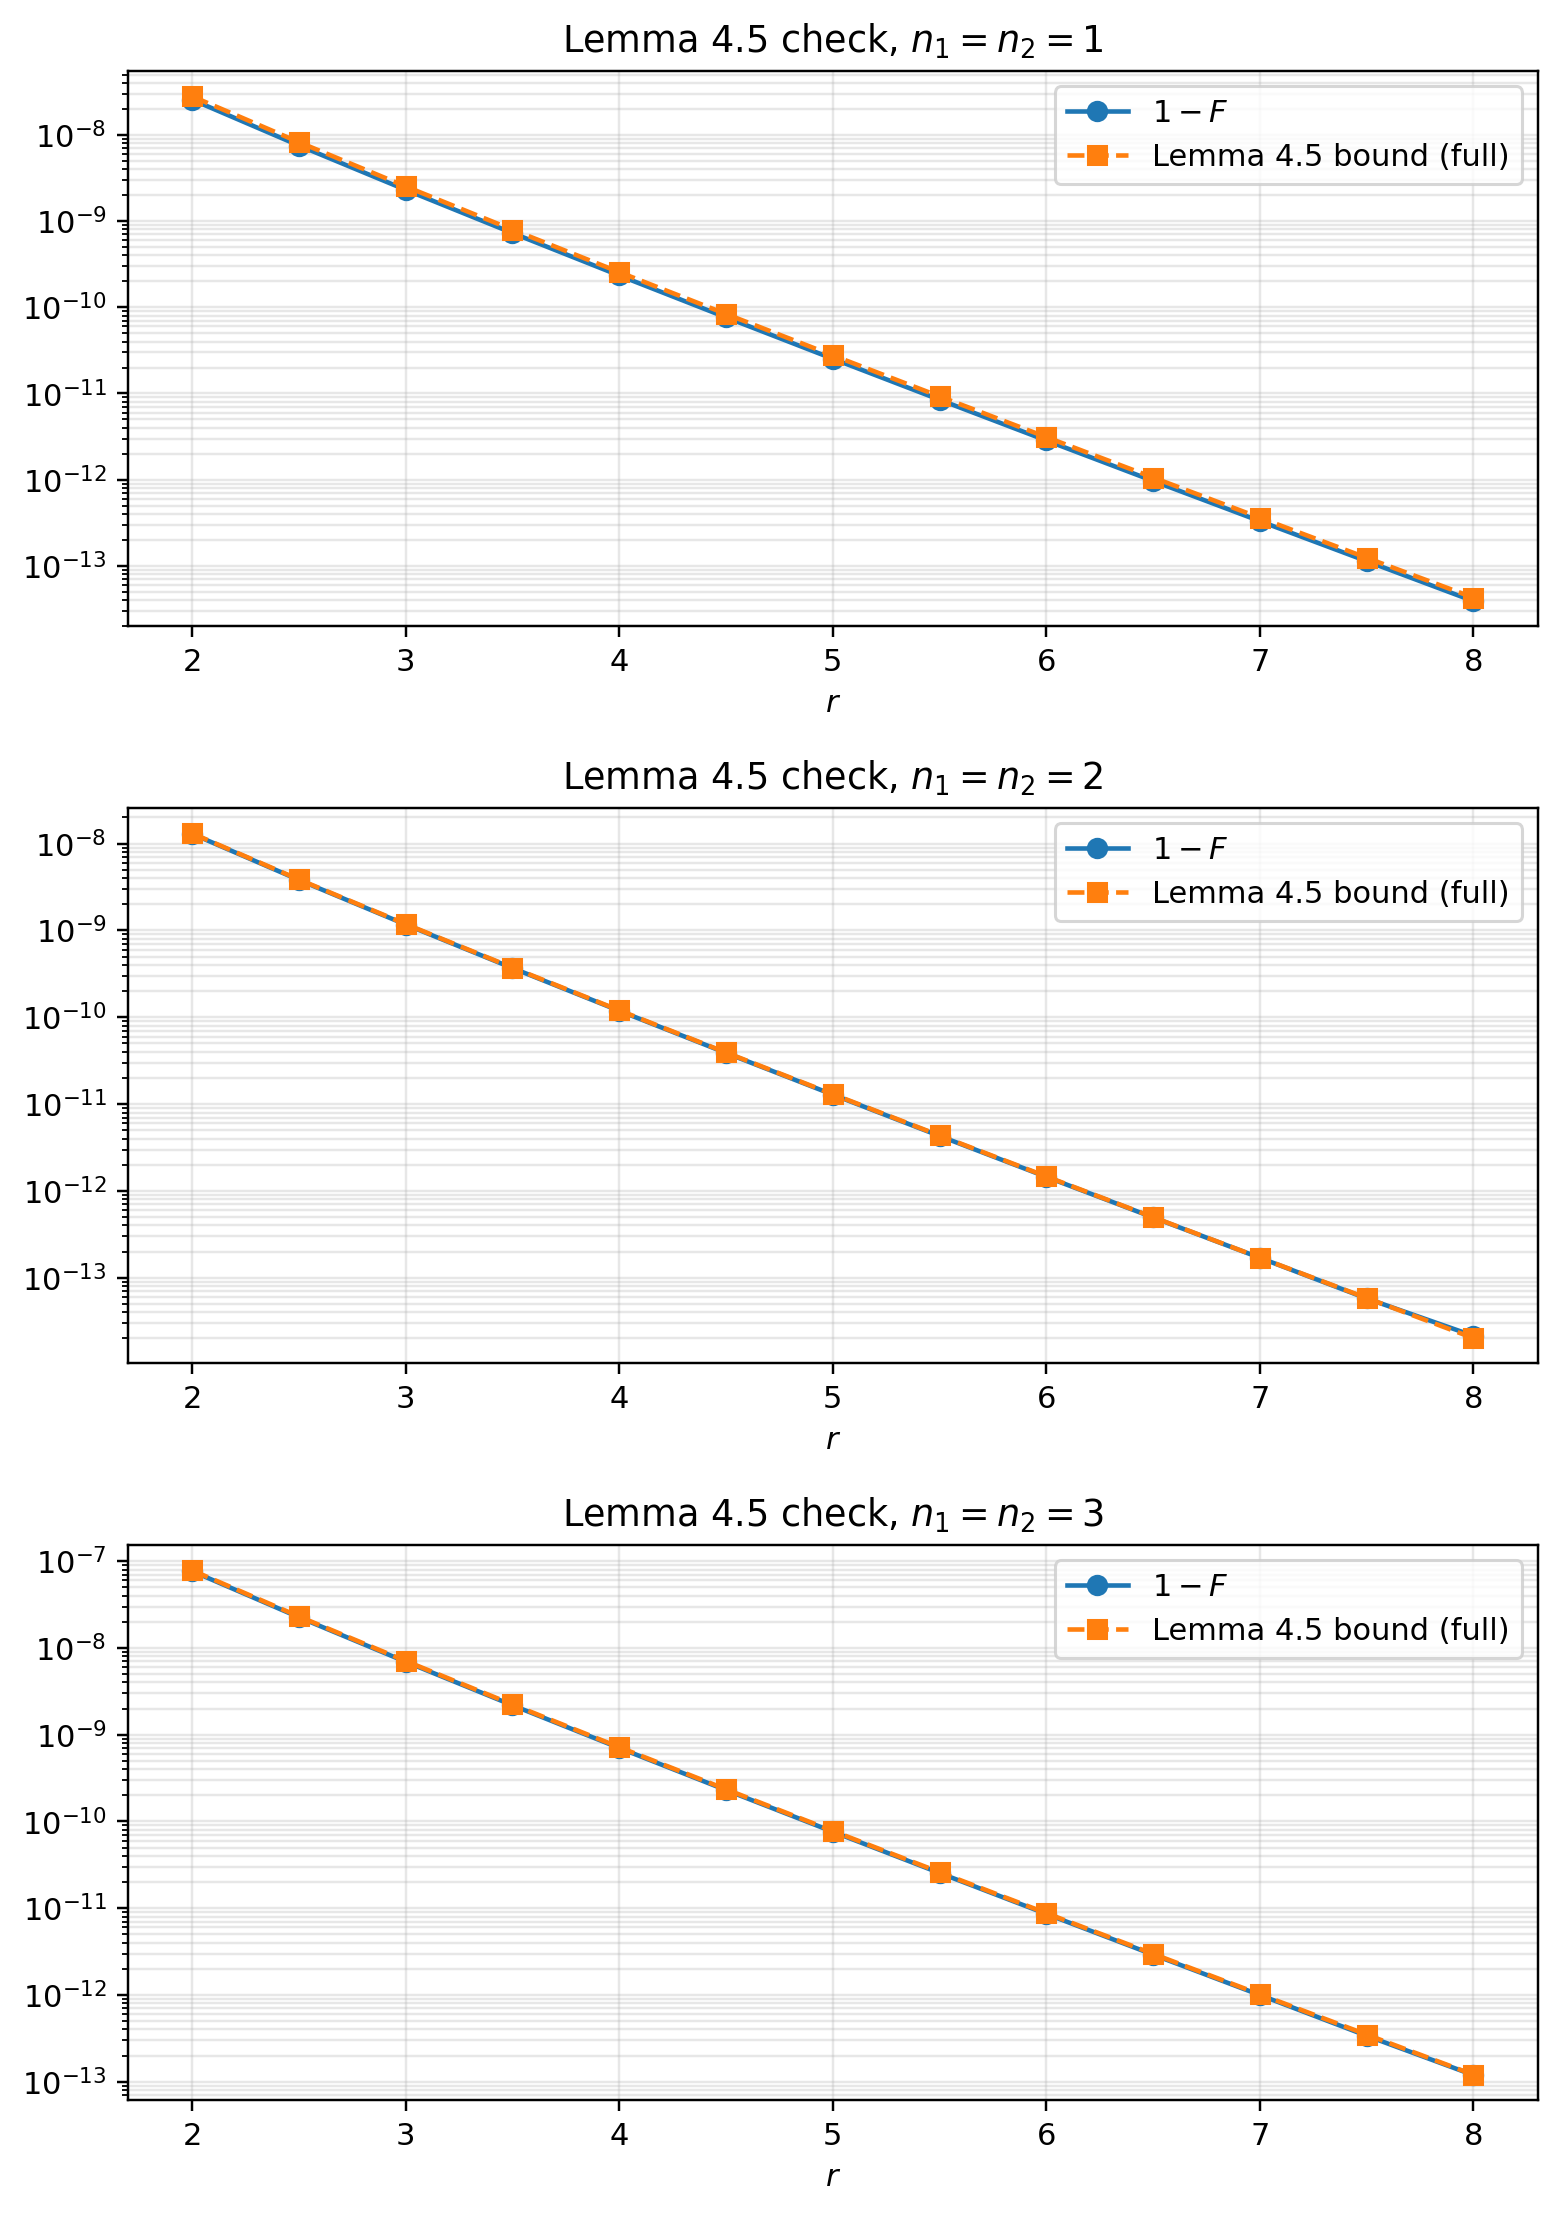
\includegraphics[width=0.75\textwidth]{fig07_dimsweep_fid.png}
\caption{N2: fidelity-benchmark comparison across $n_1=n_2\in\{1,2,3\}$.}
\end{figure}
\begin{figure}[h]
\centering
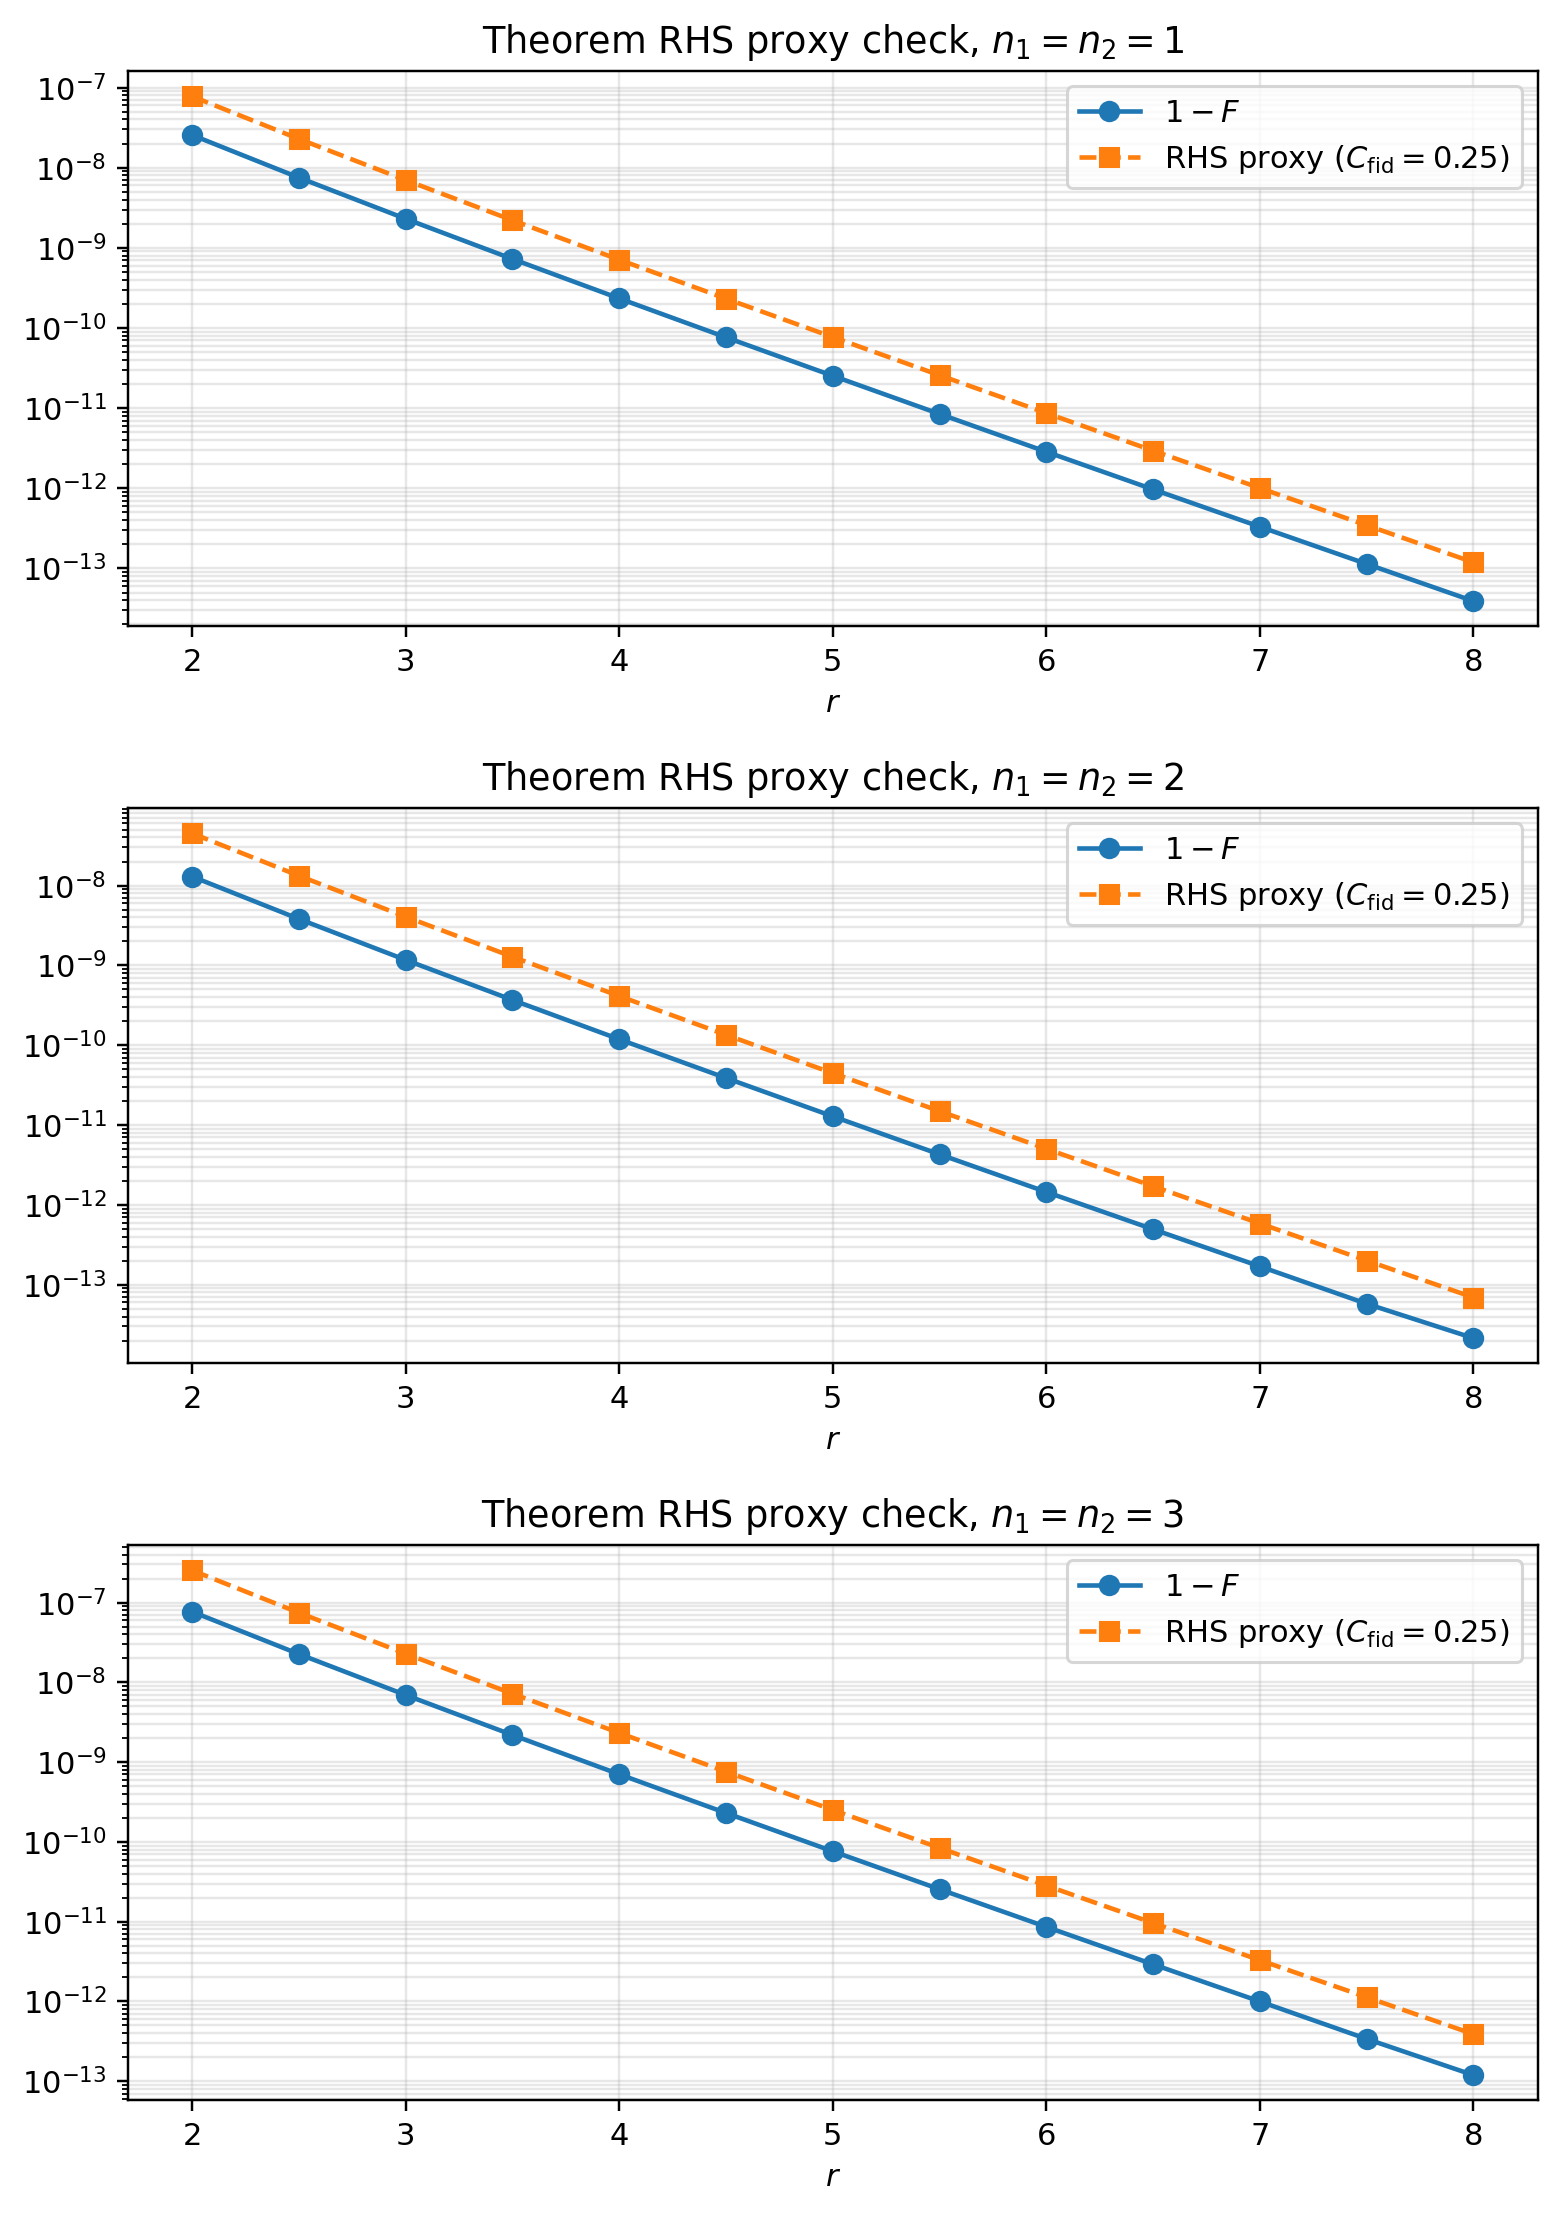
\includegraphics[width=0.75\textwidth]{fig08_dimsweep_rhs.png}
\caption{N2: $1-F$ versus the theorem RHS proxy across
$n_1=n_2\in\{1,2,3\}$.}
\end{figure}
\begin{figure}[h]
\centering
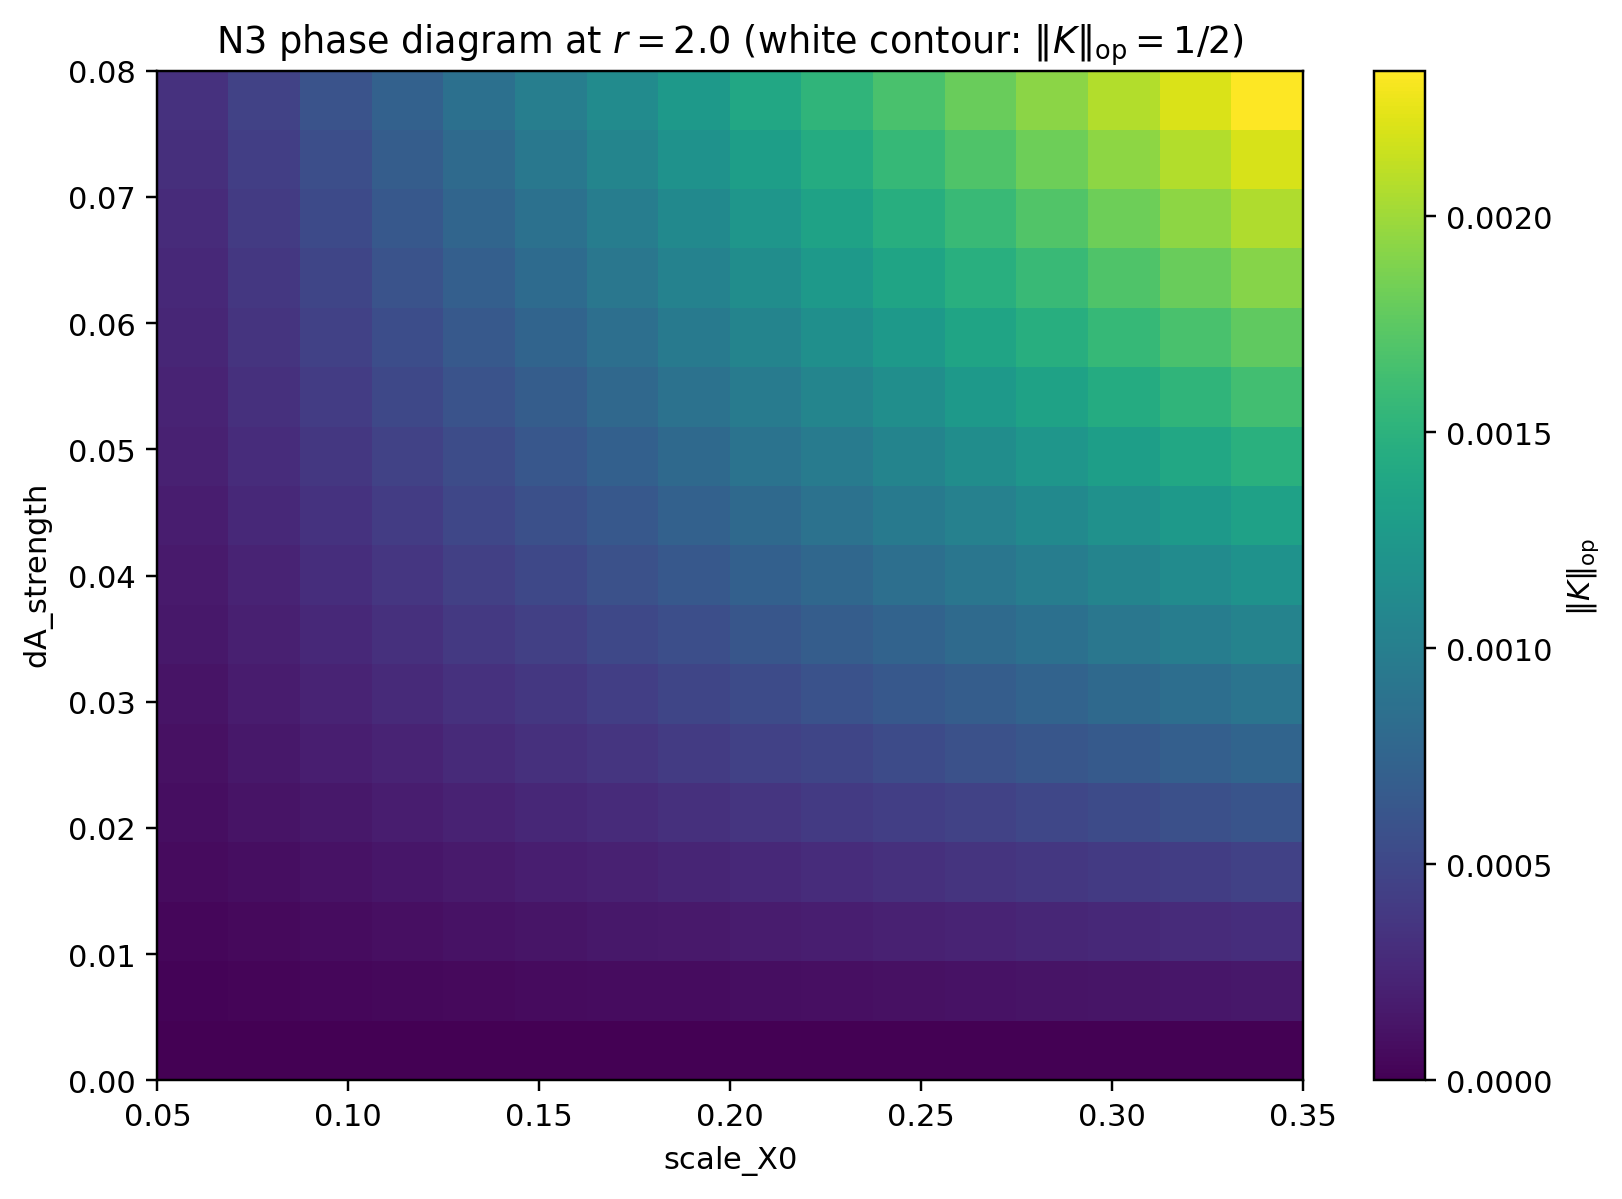
\includegraphics[width=0.7\textwidth]{fig09_heatmap_K.png}
\caption{N3 (fixed $r=2$): heatmap of $\|K\|_\op$ in a deep perturbative
region.}
\end{figure}
\begin{figure}[h]
\centering
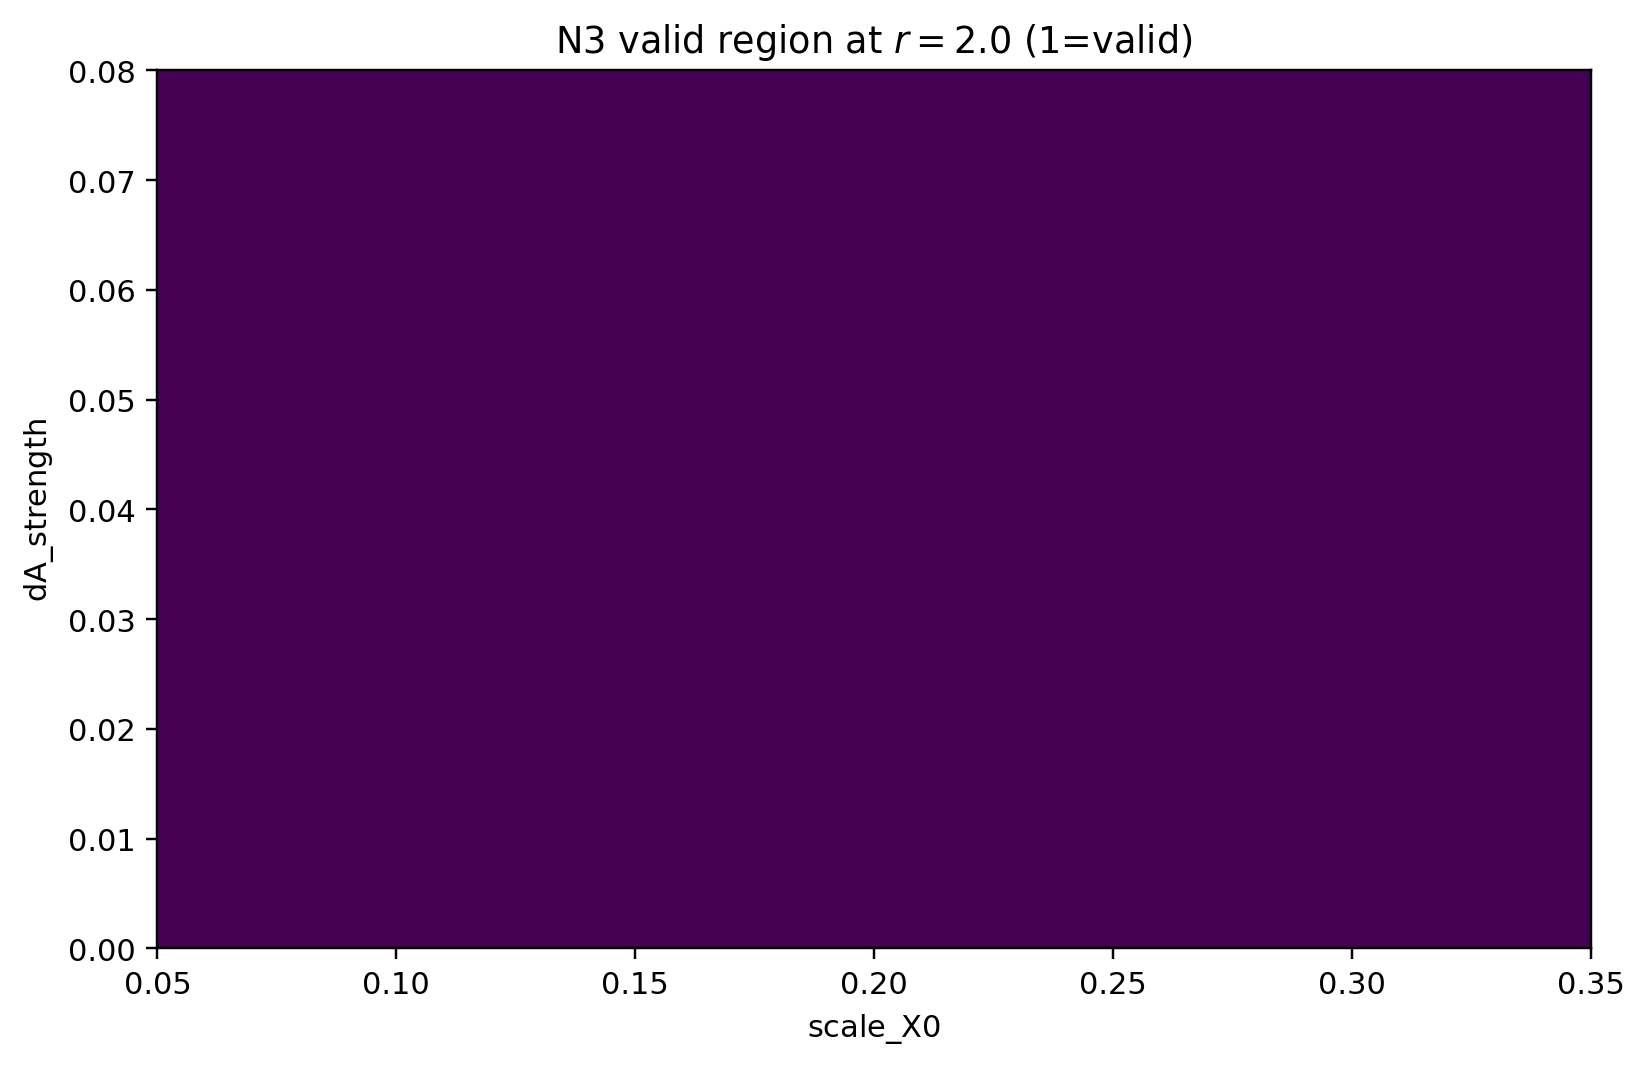
\includegraphics[width=0.7\textwidth]{fig10_validity.png}
\caption{N3 (fixed $r=2$): validity region for physicality and
$\|K\|_\op \le \frac12$.}
\end{figure}
\begin{figure}[h]
\centering
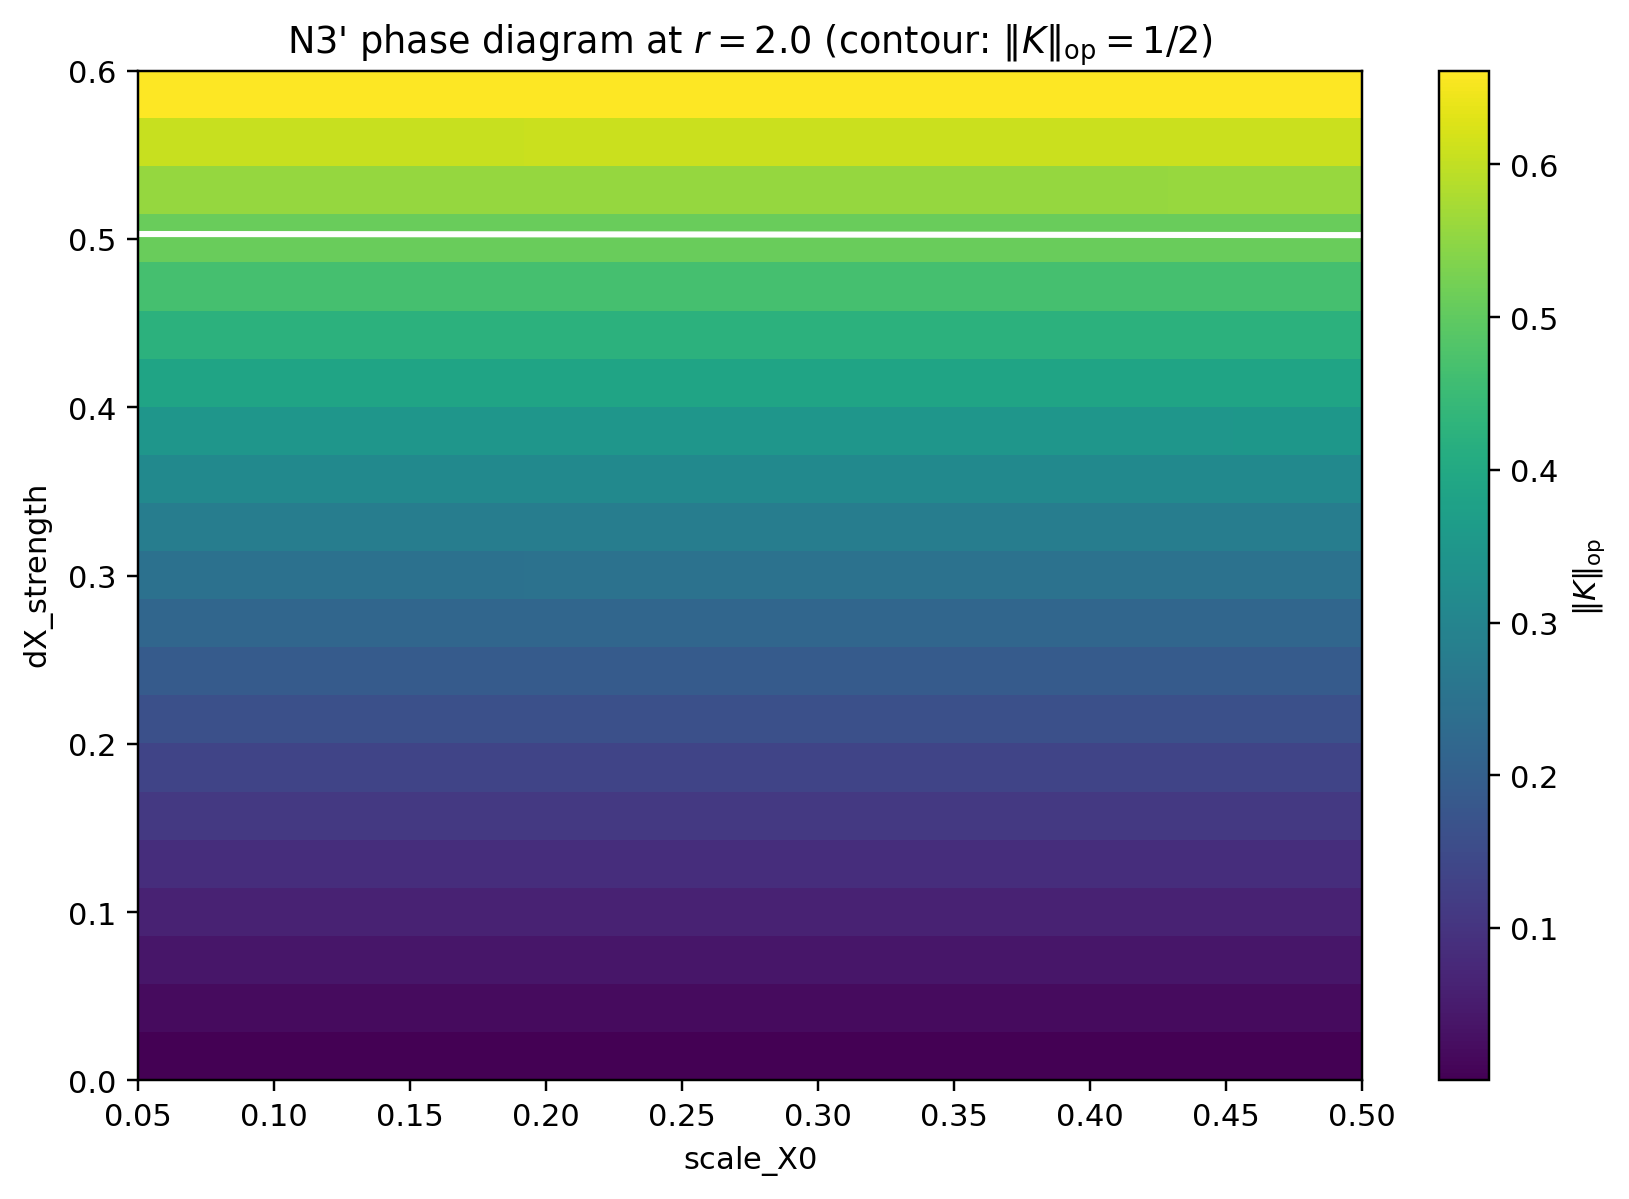
\includegraphics[width=0.7\textwidth]{fig11_phase_K.png}
\caption{N3' (fixed $r=2$): phase diagram of $\|K\|_\op$ versus scale $X_0$
and $dX$ strength; contour indicates $\|K\|_\op = \frac12$.}
\end{figure}
\begin{figure}[h]
\centering
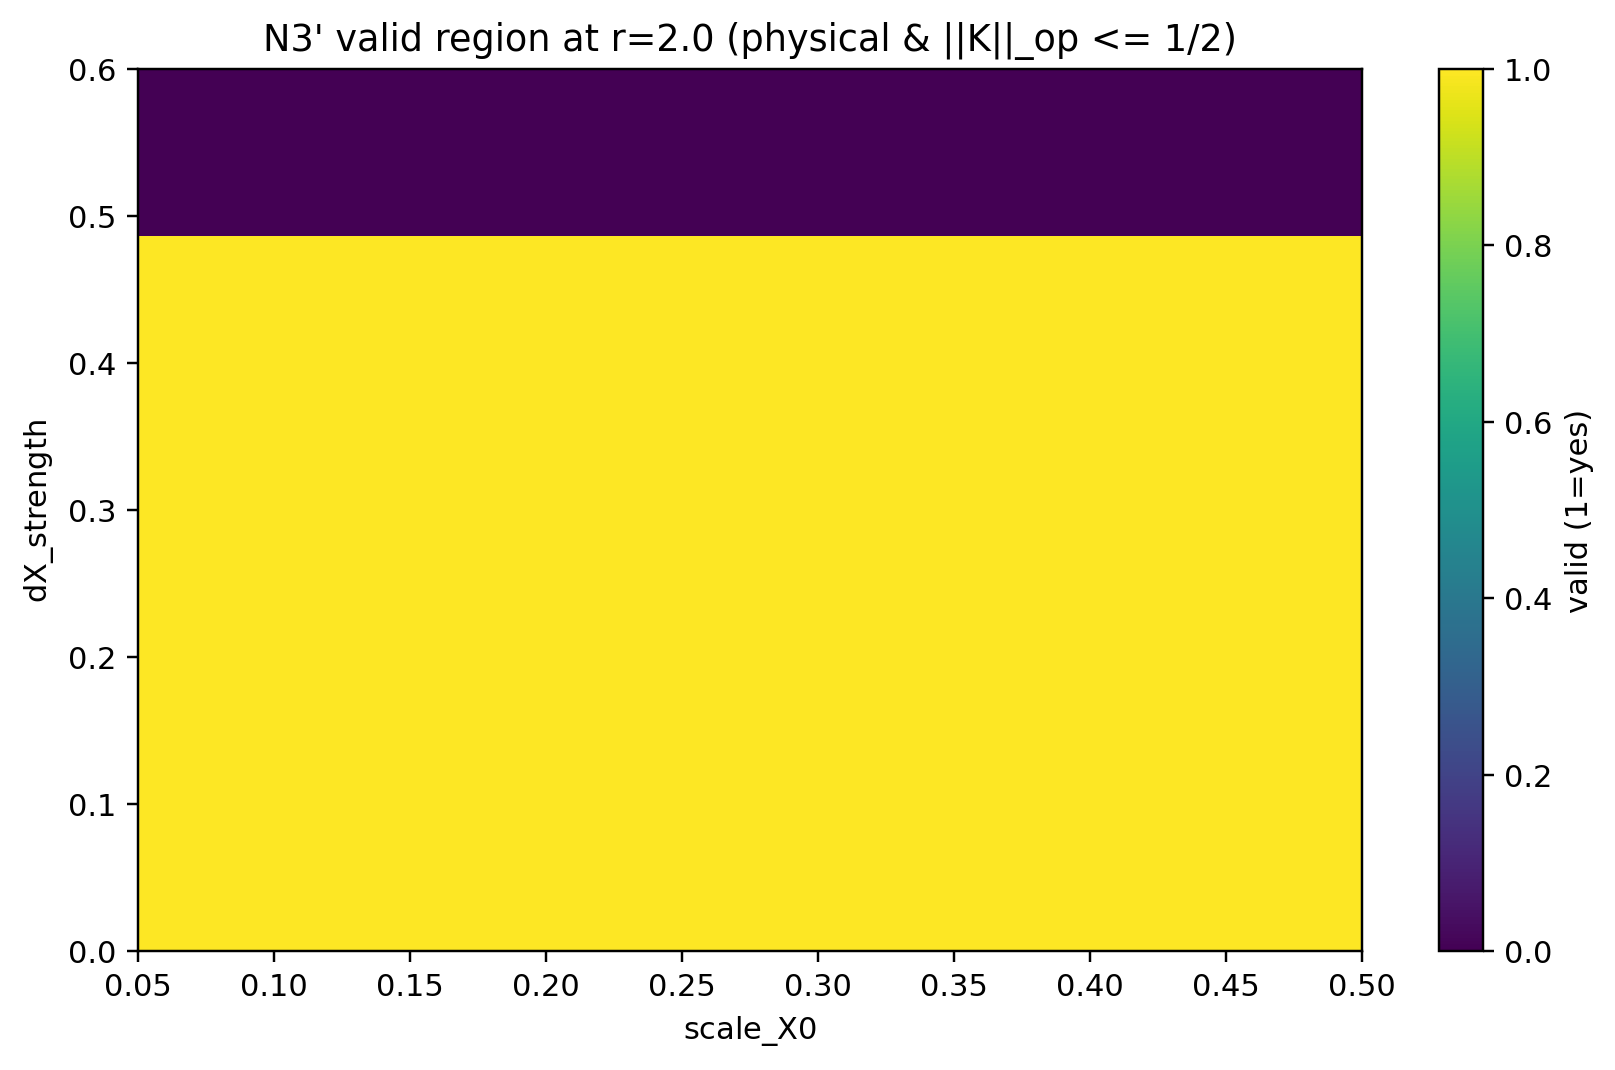
\includegraphics[width=0.7\textwidth]{fig12_phase_validity.png}
\caption{N3' (fixed $r=2$): validity region where the state remains
physical and satisfies $\|K\|_\op \le \frac12$.}
\end{figure}

\section{Appendix: verification interface (updated in v2)}
The v1 appendix carried a minimal runnable script depending on
\texttt{thewalrus==0.22.0}. In v2 it is superseded by the full suite
\texttt{verification/2601-0007/} in the series repository, consisting of
\texttt{gauss\_fid.py} (certified pure-NumPy BBP fidelity,
Remark~\ref{rem:numconv}) and \texttt{verify\_2601\_0007.py}
(Section~\ref{sec:verif}); \texttt{thewalrus}, when installed, is used only
as an optional cross-check. The recovery map and all parameter definitions
follow this paper's equations verbatim; the suite exits nonzero if any
check fails.

\begin{thebibliography}{9}
\bibitem{Petz} D. Petz, \emph{Sufficient subalgebras and the relative
entropy of states of a von Neumann algebra}, Commun. Math. Phys.
\textbf{105} (1986) 123--131.
\bibitem{FR} O. Fawzi and R. Renner, \emph{Quantum conditional mutual
information and approximate Markov chains}, Commun. Math. Phys.
\textbf{340} (2015) 575--611.
\bibitem{BBP} L. Banchi, S. L. Braunstein, and S. Pirandola, \emph{Quantum
fidelity for arbitrary Gaussian states}, Phys. Rev. Lett. \textbf{115}
(2015) 260501.
\bibitem{Weedbrook} C. Weedbrook et al., \emph{Gaussian quantum
information}, Rev. Mod. Phys. \textbf{84} (2012) 621--669.
\bibitem{Serafini} A. Serafini, \emph{Quantum Continuous Variables}, CRC
Press (2017).
\bibitem{Marian} P. Marian and T. A. Marian, \emph{Uhlmann fidelity between
two-mode Gaussian states}, Phys. Rev. A \textbf{86} (2012) 022340.
\bibitem{NIST} NIST Digital Library of Mathematical Functions, Bessel
Functions, \url{https://dlmf.nist.gov/10}.
\bibitem{Walrus} N. Killoran et al., \emph{The Walrus} (software),
\url{https://github.com/XanaduAI/thewalrus}.
\bibitem{S0060} L. Eriksson, \emph{Clustering, Recovery, and Locality in
AQFT}, ai.viXra:2512.0060 (2025; v2 2026).
\bibitem{S0101} L. Eriksson, \emph{Beyond Gaussianity: Extending the
Clustering--Recovery Bridge}, ai.viXra:2512.0101 (2025; v2 2026).
\end{thebibliography}

\end{document}
